% Compila en uno de dos formatos diferentes dependiendo del valor de ebook, el
% cual puede ser pasado por medio de una cadena de caracteres al mandar compilar
% el archivo, un ejemplo es este:
%
% pdflatex -interaction=batchmode "\newif\ifebook\ebookfalse\input{archivo.tex}"
%
% pdflatex -interaction=batchmode "\newif\ifebook\ebooktrue\input{archivo.tex}"
%
% Estas dos entradas produciran archivos diferentes con un formato especifico
\ifebook
    \documentclass[a5paper, 15pt]{book} % Papel: A5, Letra: 15pt
    \usepackage[margin=2mm]{geometry} % Margenes estrechos
    \usepackage{mathpazo} % Letra: Palatino
    \usepackage{eulervm} % Letra para matematicas: Euler
    \usepackage{wrapfig}
    \newenvironment{marginfigure} % Definicion complementaria
        {\begin{wrapfigure}{r}{0.2\textwidth}}
        {\end{wrapfigure}}
\else
    \documentclass{tufte-book} % Papel: Letter, Estilo: Tufte
    \AtBeginDocument{\fontsize{11}{15}\selectfont}
    \geometry{
    left=15mm, % left margin
    textwidth=120mm, % main text block
    marginparsep=6mm, % gutter between main text block and margin notes
    marginparwidth=60mm % width of margin notes
    }
\fi
% Paquetes a utilizar
\usepackage[spanish, es-noquoting]{babel} % Español
\usepackage[usenames,dvipsnames]{xcolor} % Nombres de colores
\usepackage[utf8]{inputenc} % Texto de entrada en UTF-8
\usepackage{amsmath}        % Paquete con definiciones matematicas
\usepackage{amsthm}         % Paquete para definir ambientes de teoremas
\usepackage{amssymb}        % Paquete con simbolos matematicos
\usepackage{xfrac}          % Paquete para usar fracciones inclinadas
\usepackage{graphicx}       % Paquete para incluir imagenes
\usepackage{bbm}            % Paquete con simbolos de campos
\usepackage{enumerate}      % Paquete para crear ambientes de listas enumeradas
\usepackage{tikz}           % Paquete para crear diagramas
\usepackage{todonotes}      % Paquete para crear anotaciones
\usepackage{mathrsfs}       % Paquete para mas simbolos de campos
\usepackage{steinmetz}      % Paquete para escribir numeros complejos
\usepackage{tcolorbox}
% Subpaquete para diagramas de bloques
\usetikzlibrary{shapes, arrows, decorations.markings}
% Estilos comunes de bloques para diagramas
\tikzstyle{input} = [coordinate]
\tikzstyle{output} = [coordinate]
\tikzstyle{init} = [pin edge={to-, thin, black}]
\tikzstyle{sum} = [draw, circle]
\tikzstyle{empty} = [coordinate]
\tikzstyle{vecArrow} = [thick, decoration={markings, mark=at position
    1 with {\arrow[semithick]{open triangle 60}}},
    double distance=1.4pt, shorten >= 5.5pt,
    preaction = {decorate},
    postaction = {draw,line width=1.4pt, white, shorten >= 4.5pt}]
\tikzstyle{innerWhite} = [semithick, white, line width=1.4pt, shorten >= 4.5pt]
% Hace que la numeración dependa del numero de capitulo
\setcounter{secnumdepth}{0}
\numberwithin{equation}{chapter}
% Definición de matriz adjunta
\newenvironment{amatrix}[1]
    {\left(\begin{array}{@{}*{#1}{c}|c@{}}}
    {\end{array}\right)}
% Definiciones de teoremas
\theoremstyle{plain}
\newtheorem{lema}{Lema}[chapter]
\newtheorem{teorema}{Teorema}[chapter]
\newtheorem{corolario}{Corolario}[chapter]
\theoremstyle{remark}
\newtheorem{nota}{Nota}[chapter]
\theoremstyle{definition}
\newtheorem{definicion}{Definición}[chapter]
\newtheorem{problema}{Problema}[chapter]
% % Opciones para colores en teoremas
% \tcbuselibrary{skins}
% % Ambiente con colores para teoremas de estilo plano
% \tcolorboxenvironment{lema}
%     {enhanced jigsaw,
%     colframe=SkyBlue,
%     interior hidden,
%     before skip=10pt,
%     after skip=10pt}
% \tcolorboxenvironment{teorema}
%     {enhanced jigsaw,
%     colframe=SkyBlue,
%     interior hidden,
%     before skip=10pt,
%     after skip=10pt}
% \tcolorboxenvironment{corolario}
%     {enhanced jigsaw,
%     colframe=SkyBlue,
%     interior hidden,
%     before skip=10pt,
%     after skip=10pt}
% % Ambiente con colores para teoremas de estilo anotacion
% \tcolorboxenvironment{nota}
%     {blanker,
%     left=5mm,
%     before skip=10pt,
%     after skip=10pt,
%     borderline west={1mm}{0pt}{Orchid}}
% % Ambiente con colores para teoremas de estilo definicion
% \tcolorboxenvironment{definicion}
%     {frame empty,
%     colback=OliveGreen!10!White,
%     grow to left by=6pt,
%     grow to right by=6pt,
%     left=1.6pt,
%     right=1.6pt,
%     arc=5pt}
% \tcolorboxenvironment{problema}
%     {frame empty,
%     colback=OliveGreen!10!White,
%     grow to left by=6pt,
%     grow to right by=6pt,
%     left=1.6pt,
%     right=1.6pt,
%     arc=5pt}
% Definiciones de operadores
\DeclareMathOperator{\rango}{rango}
\DeclareMathOperator{\imagen}{Im}
\DeclareMathOperator{\grado}{grado}
\DeclareMathOperator{\traza}{traza}
\DeclareMathOperator{\supremo}{supremo}
\DeclareMathOperator{\cardinalidad}{cardinalidad}
% Definiciones para recordatorios por hacer
\newcommand{\tarea}[2][]
    {\todo[
        linecolor=black!50!white,       % Color de linea: Gris
        backgroundcolor=black!30!white, % Color de fondo: Gris claro
        bordercolor=black!30!white,     % Color de borde: Gris claro
        #1]{#2}}
\newcommand{\faltante}[2][]
    {\todo[
        linecolor=red!50!white,        % Color de linea: Rojo
        backgroundcolor=red!30!white,  % Color de fondo: Rojo claro
        bordercolor=red!30!white,      % Color de borde: Rojo claro
        #1]{#2}}


\title{Teoría de Control}
\author{Roberto Cadena Vega}

\begin{document}
    \maketitle

    \tableofcontents
    \listoftodos

    \clearpage
    
\chapter{Criterio de Estabilidad de Routh-Hurwitz}

    \begin{equation}
        \frac{\hat{y}(s)}{\hat{R}(s)} = \frac{b_0 s^m + b_1 s^{m-1} + ... + b_{m-1} s + b_m}{a_0 s^n + a_1 s^{n-1} + ... + a_{n-1} s + a_n} = \frac{B(s)}{A(s)}
    \end{equation}

    \begin{equation}
        \frac{\hat{y}(s)}{\hat{R}(s)} = \sum{\frac{k_{1,i}}{s + \alpha_i}} + \sum{\frac{k_{2,j} + k_{3,j} \cdot s}{(s + \beta_i)^2 + {\gamma_i}^2}} ; m \leq n
    \end{equation}

    El criterio de Routh-Hurwitz determina si existen raíces en el semiplano complejo derecho cerrado.

    \newpage
    \section{Tabla de Routh}
        La tabla de Routh es un método para obtener el numero de raíces con parte real positiva que se encontraran en el polinomio característico del sistema (Ecuación~\ref{eqn:ECS}) sin tener que calcular las raíces en cuestión. Se puede dividir en cuatro pasos que se enumeran a continuación.

        \begin{equation} \label{eqn:ECS}
            A(s) = a_0 s^n + a_1 s^{n-1} + ... + a_{n-1} s + a_n = 0
        \end{equation}

        \begin{enumerate}
            \item Hipótesis
                Si \begin{math}a_0 = 0 \Rightarrow\end{math} el polinomio es de orden menor a \begin{math}n\end{math}.

                Si \begin{math}a_n = 0 \Rightarrow \exists\end{math} una raíz que es \begin{math}0 \Rightarrow A(s) = (\bar{n_0} s^{\bar{n}} + \bar{a_n} s^{\bar{n-1}} + ...) s^k \end{math}.

            \item Si existen coeficientes nulos o de diferente (cambio de) signo, entonces existen raíces con parte real positiva.\newpage
            \item Construir la tabla de Routh (Ver Cuadro~\ref{tab:Routh}).

            \begin{table}[htbp]
                \centering
                \begin{tabular}{c|c c c c c}
                    $s^n$     & $a_0$ & $a_2$ & $a_4$ & $a_6$ & ...\\
                    $s^{n-1}$ & $a_1$ & $a_3$ & $a_5$ & $a_7$ & ...\\
                    $s^{n-2}$ & $b_1$ & $b_3$ & $b_5$ & $b_7$ & ...\\
                    $s^{n-3}$ & $c_1$ & $c_3$ & $c_5$ & $c_7$ & ...\\
                    $s^{n-4}$ & $d_1$ & $d_3$ & $d_5$ & $d_7$ & ...\\
                    \vdots                                         \\
                    $s^2$ & $e_1$ & $e_2$                          \\
                    $s^1$ & $f_1$                                  \\
                    $s^0$ & $g_1$
                \end{tabular}
                \caption{\label{tab:Routh}Ejemplo de tabla de Routh.}
            \end{table}

            Donde:

            \begin{math}
            b_1 = \frac{a_1 a_2 - a_0 a_3}{a_1} , b_2 = \frac{a_1 a_4 - a_0 a_5}{a_1} , \dots
            \end{math}

            \begin{math}
            c_1 = \frac{b_1 a_3 - a_1 b_2}{b_1} , c_2 = \frac{b_1 a_5 - a_1 b_3}{b_1} , \dots
            \end{math}

            \begin{math}
            d_1 = \frac{c_1 b_2 - b_1 c_2}{c_1} , d_2 = \frac{c_1 b_3 - b_1 c_3}{c_1} , \dots
            \end{math}

            \begin{math}
            \vdots
            \end{math}

            \item El número de raíces con parte real positiva es igual al numero de cambios de signo en la primera columna(Ver Cuadro~\ref{tab:Numeros}).

            \begin{table}[htbp]
                \centering
                \begin{tabular}{c|c|}
                $s^n$     & $a_0$ \\
                $s^{n-1}$ & $a_1$ \\
                $s^{n-2}$ & $b_1$ \\
                $s^{n-3}$ & $c_1$ \\
                $s^{n-4}$ & $d_1$ \\
                \vdots & \vdots   \\
                $s^2$ & $e_1$     \\
                $s^1$ & $f_1$     \\
                $s^0$ & $g_1$
                \end{tabular}
            \caption{\label{tab:Numeros}Números en los que hay que revisar el cambio de signo.}
            \end{table}

        \end{enumerate}

    \newpage
    \section{Casos Especiales}
        \begin{enumerate}

            \item En los casos en los que un coeficiente es $0$ se puede intercambiar por un $\epsilon$ lo suficientemente pequeño para aproximar a $0$ (Véase el Cuadro~\ref{tab:Caso1}).

            \begin{math}
            A(s) = s^3 + 2 s^2 + s + 2 = 0
            \end{math}

            \begin{verbatim}
            >> A = [1 2 1 2];
            >> r = roots(A)
            r =
              -2.00000 + 0.00000i
              -0.00000 + 1.00000i
              -0.00000 - 1.00000i
            \end{verbatim}

            \begin{table}[htbp]
                \centering
                \begin{tabular}{c|c c}
                $s^3$ & $1$ & $1$ \\
                $s^2$ & $2$ & $2$ \\
                $s^1$ & $0 \approx \epsilon$ \\
                $s^0$ & $2$
                \end{tabular}
            \caption{\label{tab:Caso1}Caso Especial 1.}
            \end{table}

            \item Cuando existen cambios en los coeficientes del polinomio característico se sabe que existirán raíces con parte real positiva (Véase el cuadro~\ref{tab:Caso2}).

            \begin{math}
                A(s) = s^3 - 3 s + 2 = 0
            \end{math}

            \begin{verbatim}
            >> A = [1 0 -3 2];
            >> r = roots(A)
            r =
              -2.00000
               1.00000
               1.00000
            \end{verbatim}

            \begin{table}[htbp]
                \centering
                \begin{tabular}{c|c c}
                $s^3$ & $1$ & $-3$ \\
                $s^2$ & $0\approx\epsilon$ & $2$ \\
                $s^1$ & $-\frac{2}{\epsilon}$ & $0$ \\
                $s^0$ & $2$
                \end{tabular}
                \caption{\label{tab:Caso2}Caso Especial 2.}
            \end{table}

            \item Cuando todos los coeficientes en una linea se eliminan se puede crear un nuevo polinomio auxiliar con la linea anterior, obtener su derivada e insertar en la siguiente linea para continuar calculando la tabla (Véase el Cuadro~\ref{tab:Caso3a} y~\ref{tab:Caso3b}).

            \begin{math}
            A(s) = s^5 + 2 s^4 + 24 s^3 + 48 s^2 - 25 s - 50 = 0
            \end{math}

            \begin{math}
            p_{aux}(s) = 2 s^4 + 48 s^2 - 50
            \end{math}

            \begin{math}
            \frac{\mathrm d}{\mathrm d x} p_{aux}(s) = 8 s^3 + 96 s
            \end{math}

            \begin{verbatim}
            >> A = [1 2 24 48 -25 -50];
            >> r = roots(A)
            r =
              -0.00000 + 5.00000i
              -0.00000 - 5.00000i
               1.00000 + 0.00000i
              -2.00000 + 0.00000i
              -1.00000 + 0.00000i
            \end{verbatim}

            \begin{table}[htbp]
                \centering
                \begin{tabular}{c|c c c}
                $s^5$ & $1$ & $24$ & $-25$ \\
                $s^4$ & $2$ & $48$ & $-50$ \\
                $s^3$ & $0$ & $0$  & $0$   \\
                $s^2$ \\
                $s^1$ \\
                $s^0$
                \end{tabular}
                \caption{\label{tab:Caso3a}Caso Especial 3a.}
            \end{table}

            \begin{table}[htbp]
                \centering
                \begin{tabular}{c|c c c}
                $s^5$ & $1$ & $24$ & $-25$ \\
                $s^4$ & $2$ & $48$ & $-50$ \\
                $s^3$ & $8$ & $96$ & $0$   \\
                $s^2$ & $24$ & $-50$ & $0$ \\
                $s^1$ & $112.6$ & $0$ \\
                $s^0$ & $-50$
                \end{tabular}
                \caption{\label{tab:Caso3b}Caso Especial 3b.}
            \end{table}

        \end{enumerate}

        \begin{figure*}
            \centering
            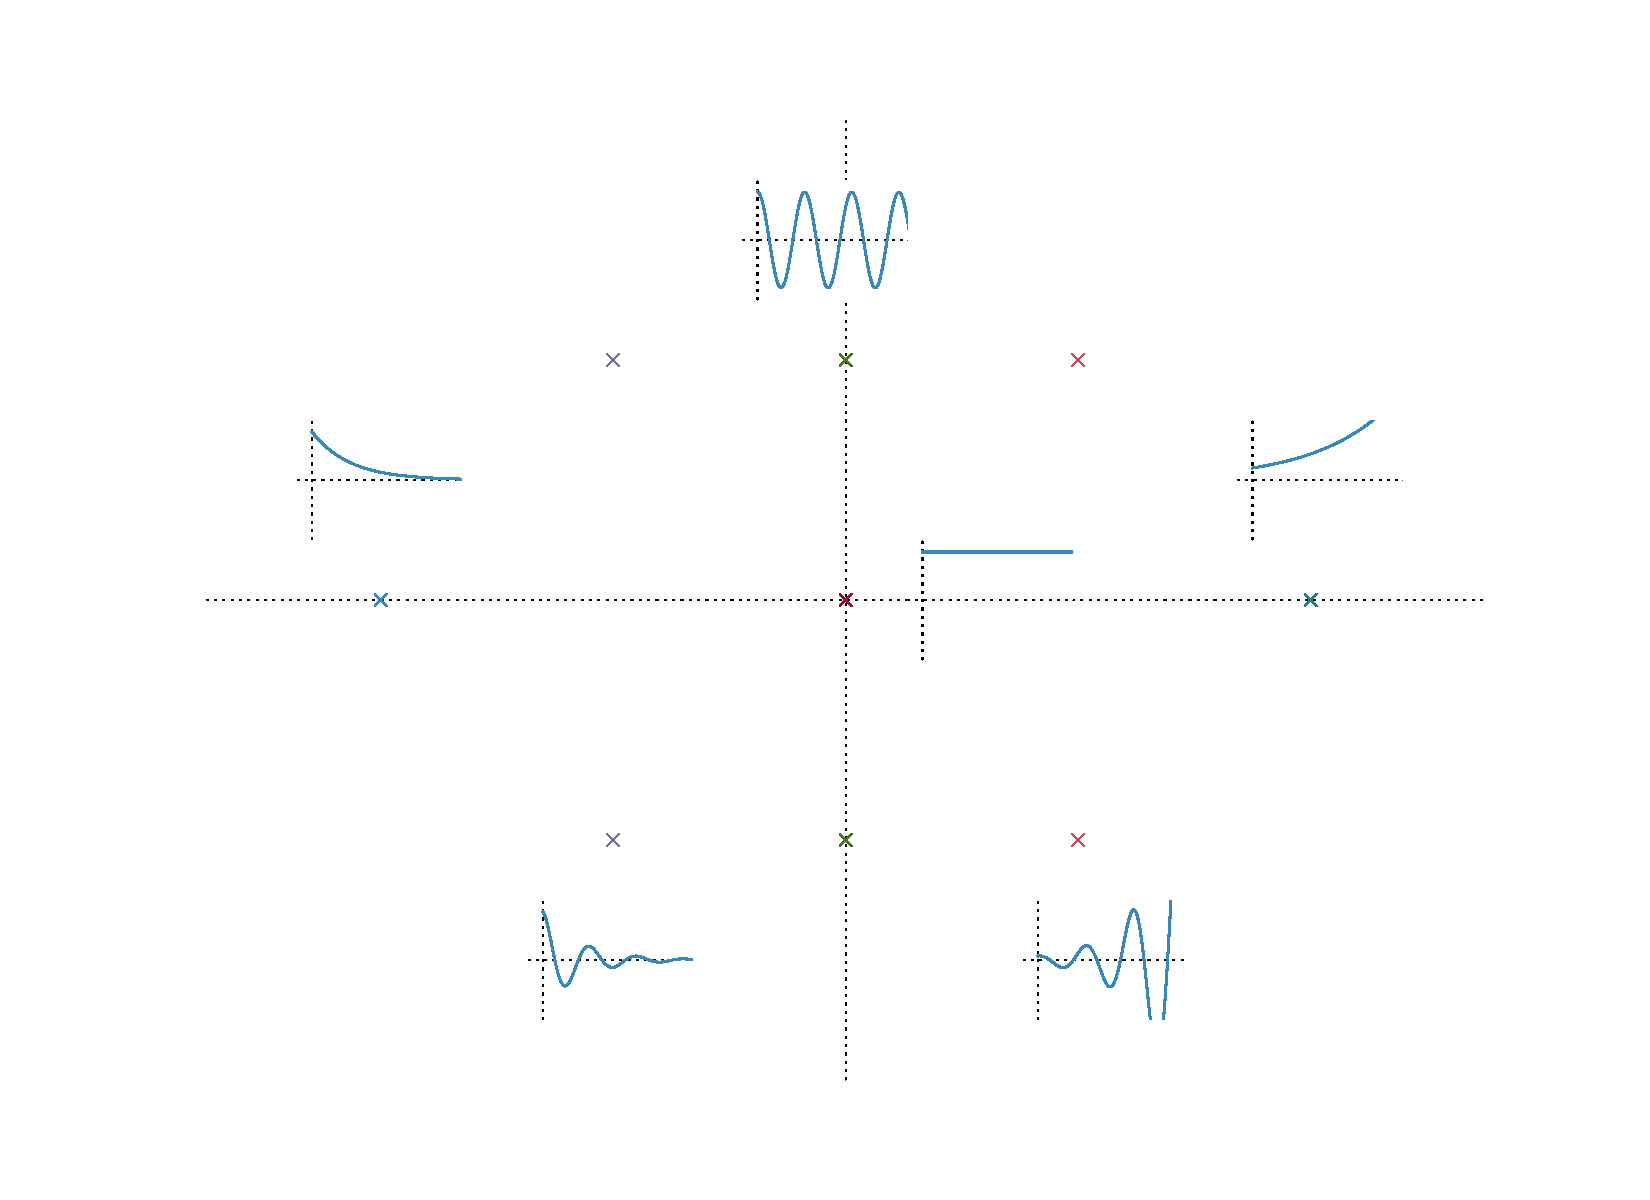
\includegraphics[width=0.9\textwidth]{./imagenes/planocomplejo.pdf}
            \caption{\label{fig:planocomplejo}Polos en el plano complejo.}
        \end{figure*}

    \newpage
    \section{Aplicación del criterio de Routh}
        Si bien los sistemas numéricos actuales permiten el calculo de las raíces de un sistema de manera mas rápida y sencilla que con la aplicación de este método, aun existen aplicaciones practicas en las que es de suma importancia el determinar el numero de raíces positivas. Por ejemplo podemos tener ganancias en un sistema para las que queremos determinar de primera instancia, un rango de valores para los cuales el sistema no se volverá inestable.

        Para ello calculamos la tabla de Routh de la misma manera en que lo hicimos anteriormente, pero teniendo en cuenta las ganancias a incluir en el calculo de las raíces (Por ejemplo con una ganancia proporcional véase Cuadro~\ref{tab:Aplicacion}).

        \begin{table}[htbp]
            \centering
            \begin{tabular}{c|c c c c c}
            $s^n$     & $a_0$ & $a_2$ & $a_4$ & $a_6$ & ...\\
            $s^{n-1}$ & $a_1$ & $a_3$ & $a_5$ & $a_7$ & $k$\\
            $s^{n-2}$ & $b_1$ & $b_3$ & $b_5$ & $b_7$ & ...\\
            $s^{n-3}$ & $c_1$ & $c_3$ & $c_5$ & $c_7$ & ...\\
            $s^{n-4}$ & $d_1$ & $d_3$ & $d_5$ & $d_7$ & ...\\
            \vdots                                         \\
            $s^2$ & $e_1$ & $e_2$                          \\
            $s^1$ & $f_1$                                  \\
            $s^0$ & $g_1$
            \end{tabular}
            \caption{\label{tab:Aplicacion}Aplicación del criterio de Routh.}
        \end{table}

        \subsection{Ejemplo:}

            \begin{figure}
                \centering
                \resizebox{\textwidth}{!}{
                    \tikzstyle{input} = [coordinate]
                    \tikzstyle{output} = [coordinate]
                    \tikzstyle{block} = [draw, rectangle, minimum height=3em, minimum width=4em]
                    \tikzstyle{sum} = [draw, circle]
                    \tikzstyle{init} = [pin edge={to-, thin, black}]

                    \begin{tikzpicture}[auto, node distance=2cm, >=latex']
                        \node [input, name=entrada] {};
                        \node [sum, right of=entrada] (suma) {$+$};
                        \node [block, right of=suma] (planta) {$\frac{k}{s(s^2 + s + 4)(s+2)}$};
                        \node [output, right of=planta] (salida) {$\hat{y}(s)$};
                        \node [block, below of=planta] (retro) {$-1$};

                        \draw [->] (entrada) -- node[name=u] {$\hat{R}(s)$} (suma);
                        \draw [->] (suma) -- (planta);
                        \draw [->] (planta) -- node[name=y] {$y$} (salida);
                        \draw [->] (y) |- (retro);
                        \draw [->] (retro) -| (suma);
                    \end{tikzpicture}}
            \end{figure}

            Se toma el sistema $\frac{\hat{y}(s)}{\hat{R}(s)} = \frac{k}{s^4 + 3 s^3 + 3 s^2 + 2 s + k}$, entonces el polinomio característico del sistema será $F(s) = s^4 + 3 s^3 + 3 s^2 + 2 s + k$.

            Construimos su tabla de Routh (Cuadro~\ref{tab:EjemploAplicacion}):

            \begin{table}[htbp]
                \centering
                \begin{tabular}{c|c c c}
                $s^4$ & $1$ & $3$ & $k$ \\
                $s^3$ & $3$ & $2$ & $0$ \\
                $s^2$ & $\frac{7}{3}$ & $k$ & $0$ \\
                $s^1$ & $2 - \frac{9}{7} k$ & $0$ \\
                $s^0$ & $k$
                \end{tabular}
                \caption{\label{tab:EjemploAplicacion}Ejemplo de Aplicación del criterio de Routh.}
            \end{table}

            De lo anterior podemos concluir que, para que no existan cambios de signos, toda la primera columna tiene que ser positiva, por lo que $k > 0$ y  $2 - ^9/_7 k > 0$, por lo que el rango de valores que puede ocupar la ganancia $k$ es $0 < k < ^{14}/_9$

            Si bien esto no nos aporta una ganancia especifica para un comportamiento deseado, si nos da la pauta a los valores a tomar en cuenta, si no se desea que el sistema sea inestable.

    \newpage
    \section{Acción Proporcional}
        Tenemos un sistema de primer orden, al que le agregaremos un controlador de ganancia proporcional y una retroalimentación negativa, por lo que las ecuaciones que describen la salida y el error del sistema quedan:

    \begin{equation}
        \frac{\hat{y}(s)}{\hat{R}(s)} = \frac{k}{Ts + 1 + k}
    \end{equation}

    \begin{equation}
        \frac{\hat{e}(s)}{\hat{R}(s)} = \frac{R(s) - Y(s)}{R(s)} = \frac{Ts + 1}{Ts + 1 + k}
    \end{equation}

        \subsection{Estabilidad}
            El problema reside en encontrar un conjunto de ganancias $k$ para las cuales el sistema es estable.
            \begin{equation}
                F(s) = s + \frac{1 + k}{T}
            \end{equation}

            Aplicamos una tabla de Routh a este polinomio característico (Cuadro~\ref{tab:AccionProporcional}).

            \begin{table}[htbp]
                \centering
                \begin{tabular}{c|c}
                $s^1$ & $1$ \\
                $s^0$ & $\frac{1+k}{T}$
                \end{tabular}
                \caption{\label{tab:AccionProporcional}Tabla de Routh para acción proporcional.}
            \end{table}

Por lo que concluimos que la ganancia $k$ debe de seguir: $k>-1$

        \subsection{Error en el estado permanente al escalón unitario}
            También es importante investigar el error que causara el controlador al introducirse. Si ponemos como señal de referencia al escalón unitario($R(s) = \frac{1}{s}$), podemos ver lo siguiente:

            \begin{math}
                \displaystyle \lim_{t \to \infty} e(t) = \lim_{s \to 0} s e(s) = \lim_{s \to 0} \frac{Ts + 1}{Ts + 1 + k} = \frac{1}{1 + k}
            \end{math}

    \newpage
    \section{Acción Integral}
        Tenemos un sistema de primer orden, al que le agregaremos un controlador de ganancia integral y una retroalimentación negativa, por lo que las ecuaciones que describen la salida y el error del sistema quedan:

        \begin{equation}
            \frac{\hat{y}(s)}{\hat{R}(s)} = \frac{k}{s(Ts + 1) + k}
        \end{equation}

        \begin{equation}
            \frac{\hat{e}(s)}{\hat{R}(s)} = \frac{R(s) - Y(s)}{R(s)} = \frac{s(Ts + 1)}{s(Ts + 1) + k}
        \end{equation}

        \subsection{Estabilidad}
            El problema reside en encontrar un conjunto de ganancias $k$ para las cuales el sistema es estable.
            \begin{equation}
                F(s) = s^2 + \frac{1}{T} s + \frac{k}{T}
            \end{equation}

            Aplicamos una tabla de Routh a este polinomio característico (Cuadro~\ref{tab:AccionIntegral}).

            \begin{table}[htbp]
                \centering
                \begin{tabular}{c|c c}
                $s^2$ & $1$ & $\frac{k}{T}$ \\
                $s^1$ & $\frac{1}{T}$ & $0$ \\
                $s^0$ & $\frac{k}{T}$
                \end{tabular}
                \caption{\label{tab:AccionIntegral}Tabla de Routh para acción integral.}
            \end{table}

            Por lo que concluimos que la ganancia $k$ debe de seguir: $k>0$

        \subsection{Error en el estado permanente al escalón unitario}
            También es importante investigar el error que causara el controlador al introducirse. Si ponemos como señal de referencia al escalón unitario($R(s) = \frac{1}{s}$), podemos ver lo siguiente:

            \begin{math}
                \displaystyle \lim_{t \to \infty} e(t) = \lim_{s \to 0} s e(s) = \lim_{s \to 0} s \left(\frac{s(Ts + 1)}{s(Ts + 1) + k} \frac{1}{s}\right) = 0
            \end{math}

    \newpage
    \section{Acción Proporcional Integral}
        \subsection{Estabilidad}
        \subsection{Error en el estado permanente al escalón unitario}


    \clearpage
    
\chapter{Lugar de las Raíces}
	Si tenemos un sistema con retroalimentación, su polinomio característico es el siguiente:

	\begin{equation}
		F(s) = 1 + H(s) G(s) = 0
	\end{equation}

	Donde $G(s)$ es la planta y $H(s)$ es el elemento de retroalimentación. Las condiciones de angulo y magnitud son las siguientes:

	\begin{equation}
		\phase{H(s) G(s)} = \pm 180^{\circ} (2R + 1) \mid R \in \mathbbm{Z}^+
	\end{equation}

	\begin{equation}
		\lvert H(s) G(s) \rvert = 1
	\end{equation}

	De aquí notamos que la condición de angulo, nos da la forma del lugar de las raíces, y la condición de magnitud nos da su posición.

	Pues bien, para trazar el lugar geométrico de las raíces seguimos una serie de pasos enumerados a continuación:

	\begin{enumerate}
		\item Determinar el lugar de las raíces en el eje real.

		Ejemplo: $H(s) = 1$, $G(s) = \frac{k}{s(s+1)(s+2)}$

		Sabemos, por una inspección visual, que los polos del sistema son $0$, $-1$, y $-2$, y que este sistema no tiene ceros. Lo cual nos indica, por la condición de angulo, que la suma de las interacciones de estas raices, nos dará la interacción total del sistema:

		\begin{equation*}
			\phase{G(s)} = - \phase{s} - \phase{s+1} - \phase{s+2} = \pm 180^{\circ} (2R + 1)
		\end{equation*}

		Notemos que cualquier lugar de las raices en el semiplano derecho complejo (inestable), viene con un angulo de $0^o$, por lo que las interacciones de cada polo serían:

		\begin{equation*}
			\phase{G(s)} = - 0^o - 0^o - 0^o = 0^o
		\end{equation*}

		lo cual obviamente no cumple con la condición de angulo del sistema.

		Si pasamos a la siguiente sección del eje real (creada por los mismos polos del sistema), tenemos que los angulos de interacción de cada polo son:

		\begin{equation*}
			\phase{G(s)} = - 180^o - 0^o - 0^o = -180^o
		\end{equation*}

		lo cual cumple con la condición de angulo del sistema.

		En la siguiente sección (entre $-1$ y $-2$), tenemos lo siguiente:

		\begin{equation*}
			\phase{G(s)} = - 180^o - 180^o - 0^o = -360^o = 0^o
		\end{equation*}

		y esto no cumple con la condición de angulo del sistema.

		En la ultima sección (entre $-2$ y $- \infty$) tenemos:

		\begin{equation*}
			\phase{G(s)} = - 180^o - 180^o - 180^o = -540^o = -180^o
		\end{equation*}

		por lo que esta ultima sección tambien es parte del lugar geométrico de las raices.

		\item Determinar las asintotas del lugar de las raíces.

		El lugar de las raices se aproxima a sus asintotas, mientras $s \to \infty$, por lo que podemos hacer una simplificación:

		\begin{equation*}
			\lim_{s \to \infty} G(s) = \lim_{s \to \infty} \frac{k}{s(s+1)(s+2)} = \lim_{s \to \infty} \frac{K}{s^3}
		\end{equation*}

		por lo que la condición de angulo queda:

		\begin{equation*}
			\phase{G(s)} = -3 \phase{s} = \pm 180^{\circ} (2R + 1) \implies \phase s = \pm 60^{\circ} (2R + 1)
		\end{equation*}

		lo cual nos da que los angulos de las asintotas son $60^o$, $-60^o$ y $120^o$.

		Por otro lado, si hacemos un proceso similar, pero con el polinomio caracteristico desarrollado, podremos ver que hay terminos mas importantes que otros, en especial cuando hacemos $s \to \infty$, por lo que:

		\begin{equation*}
			G(s) = \frac{k}{s(s+1)(s+2)} = \frac{k}{s^3 + 3 s^2 + 2 s} \approx \frac{k}{(s+1)^3}
		\end{equation*}

		por lo que podemos ver que las asintotas tienen esa forma, y que podemos asegurar que parten del punto $-1 + 0 i$.

		\item Determinar el punto de ruptura o partida de las asintotas en el eje real.

		Para determinar el punto de ruptura del lugar de las raices, tenemos que pensar en el polinomio caracteristico como la suma de 2 polinomios diferentes $A(s)$ y $B(s)$, de tal manera que ninguno contenga a la ganancia $k$, entonces tendremos:

		\begin{equation*}
			F(s) = B(s) + k A(s) = 0 \implies k = - \frac{B(s)}{A(s)}
		\end{equation*}

		implicando que estamos obteniendo las ganancias, para las cuales se tienen polos en el plano complejo.

		De aqui podemos pensar en el punto maximo de esta función de ganancias, como el punto de ruptura buscado, es decir:

		\begin{equation}
			\frac{dk}{ds} = 0
		\end{equation}

		En nuestro ejemplo, esto nos da como resultado:

		\begin{equation*}
			k = - s^3 - 3s^2 - 2 s \implies \frac{dk}{ds} = -3 s^2 + 6 s + 2 = 0
		\end{equation*}

		de donde obtenemos un par de respuestas $s_1 = -0.423$ y $s_2 = -1.577$, con ganancias asociadas $k_1 = 0.385$ y $k_2 = -0.385$.

		De aqui podemos descartar $s_2$ ya que no se encuentra en el lugar de las raices del eje real, y obviamente no puede partir de ahi, si no existe en ese lugar en especifico.

		\item Determinar los puntos donde el lugar de las raíces atraviesa el eje imaginario.

		Ya hemos visto que los polos sobre el eje real no cruzan el eje imaginario, ahora solo tenemos que encontrar las ganancias criticas, es decir, cuando los polos estan sobre el eje imaginario.

		\begin{equation*}
			F(s) = s^3 + 3 s^2 + 2 s + k
		\end{equation*}

		\begin{table}[htbp]
			\centering
			\begin{tabular}{c|c c c c c}
				$s^3$ & $1$ & $2$ \\
				$s^2$ & $3$ & $k$ \\
				$s^1$ & $2 - \sfrac{k}{3}$ & $0$ \\
				$s^0$ & $k$
			\end{tabular}
		\end{table}

		De donde obtenemos que $k > 0$, lo cual ocurre en el polo del origen  y $k < 6$, que es justo cuando cruza por el eje imaginario.

		Ahora, tan solo tenemos que obtener las raices del polinomio caracteristico con la ganancia adecuada y obtendremos el punto de cruce, alternativamente, podemos usar el polinomio auxiliar de la tabla de Routh, usaremos el correspondiente a $s^2$.

		\begin{equation*}
			P_{aux} = 3 s^2 + k = 3 s^2 + 6 = 0 \implies s = \pm \sqrt{2} j
		\end{equation*}

	\end{enumerate}


    \clearpage
    %-------------------------------------------------------------------------------
%	EMPIEZA CAPITULO
%-------------------------------------------------------------------------------

\chapter{Compensador Adelanto/Atraso (LR)}

    El concepto de fase surge del análisis del lugar de las raices, al pensar que el angulo que tiene un conjunto de raices complejas conjugadas con respecto al eje real positivo es la fase, es decir, el angulo del fasor. De esta manera, podemos modificar el comportamiento de un sistema agregando dinámicas al sistema ayudandolo a mover el lugar geométrico de las raices hacia donde lo necesitemos.

    El adelanto de fase pues, será un comportamiento demasiado rápido y subamortiguado y el atraso de fase demasiado lento y sobreamortiguado, por lo que agregaremos polos que atraigan el lugar de las raices y que modifiquen la fase para adelantarla (si es un comportamiento demasiado lento o sobreamortiguado) o atrasarla (si es un comportamiento demasiado rapido o subamortiguado).

    Empezaremos considerando el siguiente sistema como base para nuestros calculos:

    \begin{figure}
        \centering
        \resizebox{0.6\textwidth}{!}{
            \tikzstyle{block} = [draw, rectangle, minimum height=3em, minimum width=4em]
            \tikzstyle{sum} = [draw, circle]

            \begin{tikzpicture}[auto, node distance=2cm, >=latex']
                \node [input, name=entrada] {};
                \node [sum, right of=entrada] (suma) {$+$};
                \node [block, right of=suma] (ganancia) {$k$};
                \node [block, right of=ganancia] (planta) {$G(s)$};
                \node [output, right of=planta] (salida) {};
                \node [block, below of=planta] (retro) {$-1$};

                \draw [->] (entrada) -- node[name=u] {$r(s)$} (suma);
                \draw [->] (suma) -- (ganancia);
                \draw [->] (ganancia) -- (planta);
                \draw [->] (planta) -- node[name=y] {$y(s)$} (salida);
                \draw [->] (y) |- (retro);
                \draw [->] (retro) -| (suma);
            \end{tikzpicture}}
        \caption{\label{dia:caa1}Planta con controlador proporcional y realimentación unitaria.}
    \end{figure}

%-------------------------------------------------------------------------------
%	EMPIEZA SECCION
%-------------------------------------------------------------------------------

    \newpage
    \section{Compensador de adelanto de fase}

        Dado el siguiente sistema realimentado:

        \begin{figure}
            \centering
            \resizebox{0.6\textwidth}{!}{
                \tikzstyle{block} = [draw, rectangle, minimum height=3em, minimum width=4em]
                \tikzstyle{sum} = [draw, circle]

                \begin{tikzpicture}[auto, node distance=2cm, >=latex']
                    \node [input, name=entrada] {};
                    \node [sum, right of=entrada] (suma) {$+$};
                    \node [block, right of=suma] (ganancia) {$G_c(s)$};
                    \node [block, right of=ganancia] (planta) {$G(s)$};
                    \node [output, right of=planta] (salida) {};
                    \node [block, below of=planta] (retro) {$-1$};

                    \draw [->] (entrada) -- node[name=u] {$r(s)$} (suma);
                    \draw [->] (suma) -- (ganancia);
                    \draw [->] (ganancia) -- (planta);
                    \draw [->] (planta) -- node[name=y] {$y(s)$} (salida);
                    \draw [->] (y) |- (retro);
                    \draw [->] (retro) -| (suma);
                \end{tikzpicture}}
            \caption{\label{dia:caa2}Planta con compensador y realimentación unitaria.}
        \end{figure}

        Tenemos que el controlador es de la forma:

        \begin{equation}
            G_c(s) = k_c \alpha \frac{Ts + 1}{\alpha T s + 1} = \hat{k}_c \frac{s + \frac{1}{T}}{s + \frac{1}{\alpha T}}
        \end{equation}

        con $k_c > 0$ y $0 < \alpha < 1$.

        Dadas estas condiciones, el lugar de las raíces de los polos y ceros\footnote{El cero atrae el lugar de las raices hacia la izquierda.} agregados se verán como en la figura.

        \begin{marginfigure}
            \centering
            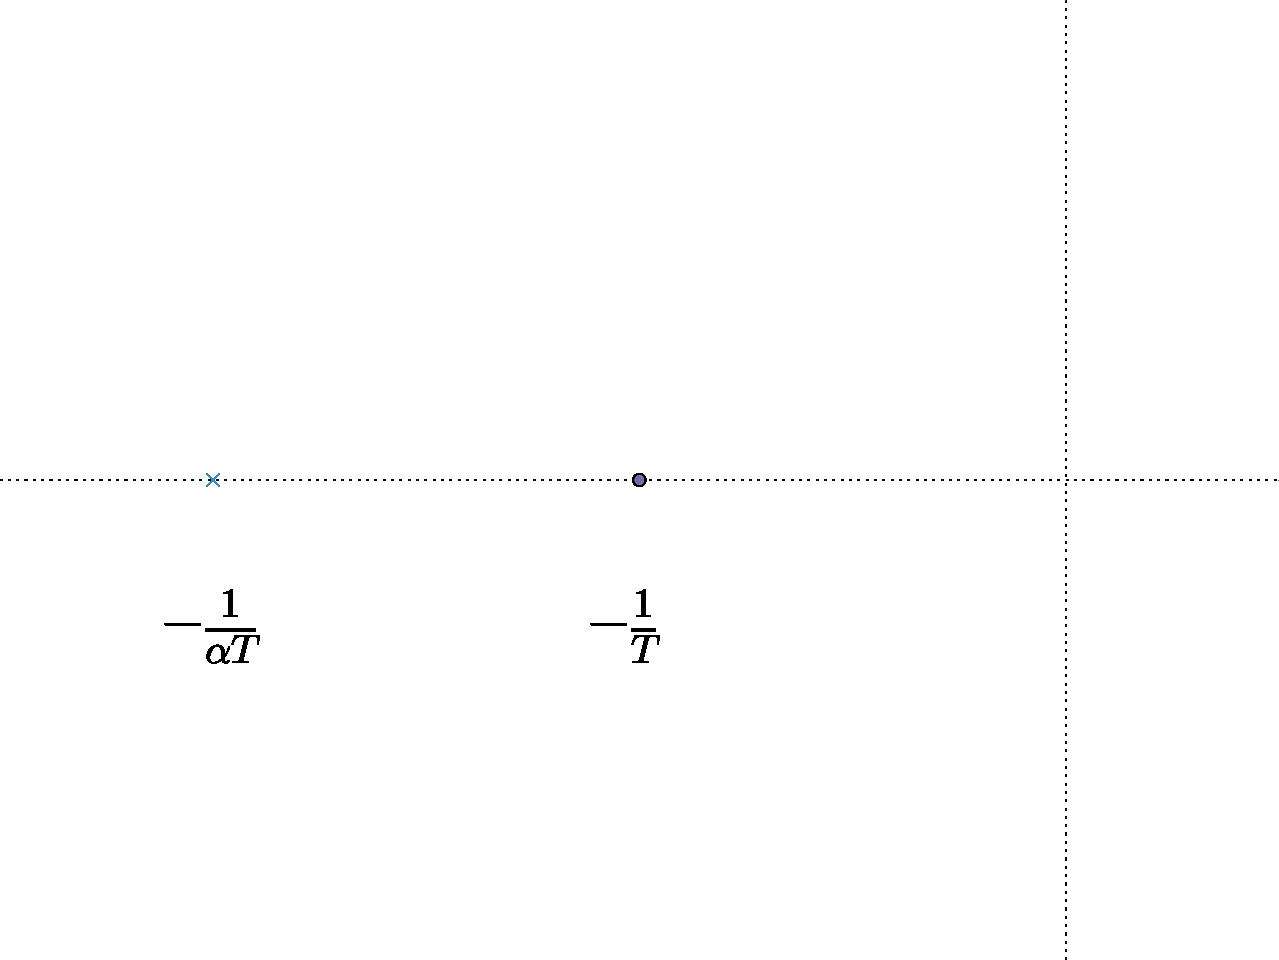
\includegraphics[width=\textwidth]{./imagenes/adelantopoloycero.pdf}
            \caption{\label{fig:adelantopoloycero}Polo y cero introducidos por el compensador de adelanto de fase.}
        \end{marginfigure}

        Dado este controlador se pueden modificar el comportamiento del sistema para hacerlo tan rápido como sea necesario. El calculo de los parametros $T$ y $\alpha$ será explicado con un ejemplo.

%-------------------------------------------------------------------------------

        \subsection{Ejemplo}
        \faltante{Falta escribir apunte}

%-------------------------------------------------------------------------------
%	EMPIEZA SECCION
%-------------------------------------------------------------------------------

    \newpage
    \section{Compensador de atraso de fase}

        Dado el siguiente sistema realimentado:

        \begin{figure}
            \centering
            \resizebox{0.6\textwidth}{!}{
                \tikzstyle{block} = [draw, rectangle, minimum height=3em, minimum width=4em]
                \tikzstyle{sum} = [draw, circle]

                \begin{tikzpicture}[auto, node distance=2cm, >=latex']
                    \node [input, name=entrada] {};
                    \node [sum, right of=entrada] (suma) {$+$};
                    \node [block, right of=suma] (ganancia) {$G_c(s)$};
                    \node [block, right of=ganancia] (planta) {$G(s)$};
                    \node [output, right of=planta] (salida) {};
                    \node [block, below of=planta] (retro) {$-1$};

                    \draw [->] (entrada) -- node[name=u] {$r(s)$} (suma);
                    \draw [->] (suma) -- (ganancia);
                    \draw [->] (ganancia) -- (planta);
                    \draw [->] (planta) -- node[name=y] {$y(s)$} (salida);
                    \draw [->] (y) |- (retro);
                    \draw [->] (retro) -| (suma);
                \end{tikzpicture}}
            \caption{\label{dia:caa3}Planta con ccompensador y realimentación unitaria.}
        \end{figure}

        Tenemos que el controlador es de la forma:

        \begin{equation}
            G_c(s) = k_c \beta \frac{Ts + 1}{\beta T s + 1} = \hat{k}_c \frac{s + \frac{1}{T}}{s + \frac{1}{\beta T}}
        \end{equation}

        con $k_c > 0$ y $\beta > 1$.

        Dadas estas condiciones, el lugar de las raíces de los polos y ceros agregados se verán como en la figura.

        \begin{marginfigure}
            \centering
            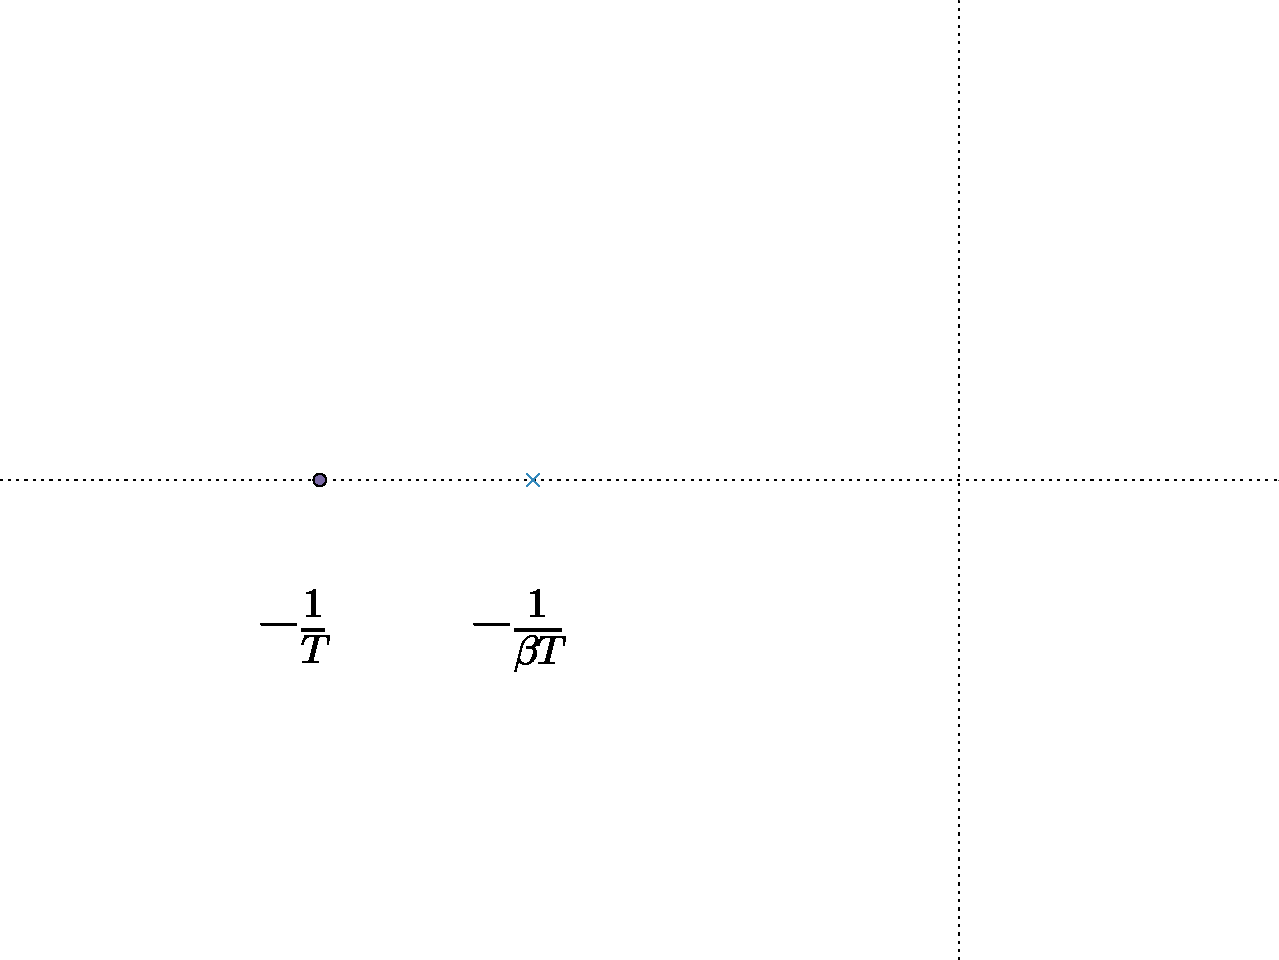
\includegraphics[width=\textwidth]{./imagenes/atrasopoloycero.pdf}
            \caption{\label{fig:atrasopoloycero}Polo y cero introducidos por el compensador de atraso de fase.}
        \end{marginfigure}

        Si el cero y el polo están muy cercanos, entonces para $s=s_1$ un polo dominante en lazo cerrado, se tiene que la magnitud del sistema:

        \begin{equation*}
            \left| G_c(s_1) \right| = \left| \hat{k}_c \frac{s_1 + \frac{1}{T}}{s_1 + \frac{1}{\beta  T}} \right| \approx \left| \hat{k}_c \right|
        \end{equation*}

        y en especifico para la fase:

        \begin{equation*}
            -5^o < \phase{\frac{s_1 + \frac{1}{T}}{s_1 + \frac{1}{\beta  T}}} < 0^o
        \end{equation*}

        Por lo que se puede aumentar la ganancia en el polo del sistema, sin sufrir un corrimiento considerable en el lugar de las raíces.

%-------------------------------------------------------------------------------

        \subsection{Error estático de posición $k_p$}

            Para el sistema dado:

            \begin{figure}
                \centering
                \resizebox{0.6\textwidth}{!}{
                    \tikzstyle{block} = [draw, rectangle, minimum height=3em, minimum width=4em]
                    \tikzstyle{sum} = [draw, circle]

                    \begin{tikzpicture}[auto, node distance=2cm, >=latex']
                        \node [input, name=entrada] {};
                        \node [sum, right of=entrada] (suma) {$+$};
                        \node [block, right of=suma] (planta) {$G(s)$};
                        \node [output, right of=planta] (salida) {};
                        \node [block, below of=planta] (retro) {$-1$};

                        \draw [->] (entrada) -- node[name=u] {$r(s)$} (suma);
                        \draw [->] (suma) -- (planta);
                        \draw [->] (planta) -- node[name=y] {$y(s)$} (salida);
                        \draw [->] (y) |- (retro);
                        \draw [->] (retro) -| (suma);
                    \end{tikzpicture}}
                \caption{\label{dia:caa4}Planta con realimentación unitaria.}
            \end{figure}

            con una entrada de tipo escalón:

            \begin{equation*}
                r(s) = \frac{1}{s}
            \end{equation*}

            y un sistema $G(s)$:

            \begin{equation*}
                G(s) = k_p \frac{s + \frac{1}{T}}{s + \frac{1}{\beta T}}
            \end{equation*}

            El error en estado permanente a una entrada escalón unitario es:

            \begin{equation*}
                e_{ss} = \lim_{s \to 0} s \left( \frac{1}{1 + G(s)} \frac{1}{s} \right) = \lim_{s \to 0} \frac{1}{1 + G(s)} = \frac{1}{1 + G(0)} = \frac{1}{1 + k_p}
            \end{equation*}

            \missingfigure{Gráfica de escalon unitario con error en estado estacionario.}

%-------------------------------------------------------------------------------

        \subsection{Error estático de velocidad $k_v$}
            El error en estado permanente a una entrada rampa unitaria es:

            \begin{equation*}
                r(s) = \frac{1}{s^2}
            \end{equation*}

            \begin{equation*}
                e_{ss} = \lim_{s \to 0} s \left( \frac{1}{a + G(s)} \frac{1}{s^2} \right) = \lim_{s \to 0} \frac{1}{s + s G(s)} = \lim_{s \to 0} \frac{1}{s G(s)} = \frac{1}{k_v}
            \end{equation*}

            \begin{equation*}
                k_v = \lim_{s \to 0} s G(s)
            \end{equation*}

            \missingfigure{Gráfica de rampa unitaria con error en estado estacionario.}

%-------------------------------------------------------------------------------

        \subsection{Ejemplo}
        \faltante{Falta escribir apunte}


    \clearpage
    
\chapter{Diagramas de Bode}

    Dado el siguiente sistema:

    \begin{figure}
        \centering
        \resizebox{0.6\textwidth}{!}{
            \tikzstyle{input} = [coordinate]
            \tikzstyle{output} = [coordinate]
            \tikzstyle{block} = [draw, rectangle, minimum height=3em, minimum width=4em]
            \tikzstyle{sum} = [draw, circle]
            \tikzstyle{init} = [pin edge={to-, thin, black}]

            \begin{tikzpicture}[auto, node distance=2cm, >=latex']
                \node [input, name=entrada] {};
                \node [block, right of=entrada] (planta) {$G(s)$};
                \node [output, right of=planta] (salida) {};

                \draw [->] (entrada) -- node[name=u] {$x(s)$} (planta);
                \draw [->] (planta) -- node[name=y] {$y(s)$} (salida);
            \end{tikzpicture}}
    \end{figure}

    con $G(s)$ Hurwitz estable:

    \begin{equation*}
        y(s) = G(s) x(s)
    \end{equation*}

    asumimos que la entrada es de la forma:

    \begin{equation*}
        x(s) = X \left( \frac{\omega}{s^2 + \omega^2} \right)
    \end{equation*}

    y la planta es de la forma:

    \begin{equation*}
        G(s) = \frac{p(s)}{q(s)} = \frac{p(s)}{(s + s_1) (s + s_2) \dots (s + s_n)}
    \end{equation*}

    de donde se asumen polos simples de primero orden, aunque los reslutados por obtener se mantienen si los polos no lo son.

    Al sustituir pues en la ecuación del sistema, tendremos:

    \begin{eqnarray*}
        y(s) & = & X \left( \frac{\omega}{s^2 + \omega^2} \right) \frac{p(s)}{(s + s_1) (s + s_2) \dots (s + s_n)} \\
        & = & \frac{a}{s + j \omega} + \frac{\bar{a}}{s - j \omega} + \frac{b_1}{s + s_1} + \dots + \frac{b_n}{s + s_n}
    \end{eqnarray*}

    lo cual podemos resolver obteniendo la transformada inversa de Laplace:

    \begin{equation*}
        y(t) = a e^{-j \omega t} + \bar{a} e^{j \omega t} + b_1 e^{-s_1 t} + \dots + b_n e^{-s_n t}
    \end{equation*}

    lo cual implica que tendremos una salida en estado estacionario:

    \begin{equation*}
        y_{ss}(t) = \lim_{t \to \infty} y(t) = a e^{-j \omega t} + \bar{a} e ^{j \omega t}
    \end{equation*}

    es decir, cuando $t$ tiende a $\infty$ todos los polos del sistema se eliminan y nos queda el comportamiento de la entrada a seguir.

    Por otro lado, para obtener los valores de $a$ y $\bar{a}$ aplicamos fracciones parciales y obtenemos:

    \begin{eqnarray*}
        a & = & \left. G(s) X \left( \frac{\omega}{s^2 + \omega^2} \right) + (s + j \omega) \right|_{s=-j \omega} = - G(-j \omega) X \frac{1}{2j} \\
        \bar{a} & = & \left. G(s) X \left( \frac{\omega}{s^2 + \omega^2} \right) + (s - j \omega) \right|_{s=j \omega} = G(j \omega) X \frac{1}{2j}
    \end{eqnarray*}

    de donde sabemos que $G(j \omega)$ lo podemos escribir como su magnitud multiplicado por una exponencial de mangitud unitaria con el angulo deseado:

    \begin{eqnarray*}
        G(j \omega) & = & \left| G(j \omega) \right| e^{j \phi} \\
        G(-j \omega) & = & \left| G(j \omega) \right| e^{-j \phi}
    \end{eqnarray*}

    en donde $\phi = \phase{G(j \omega)} = \arctan{\left( \frac{\Im{G}}{\Re{G}} \right)}$.

    Por lo tanto, $a$ y $\bar{a}$ los podemos escribir como:

    \begin{eqnarray*}
        a & = & - \left| G(j \omega) \right| e^{-j \phi} X \frac{1}{2j} \\
        \bar{a} & = & \left| G(j \omega) \right| e^{j \phi} X \frac{1}{2j}
    \end{eqnarray*}

    Tomando esto en cuenta, la salida en estado estacionario nos quedará:

    \begin{eqnarray*}
        y_{ss}(t) & = & X \left| G(j \omega) \right| \frac{e^{j(\omega t + \phi)} - e^{-j(\omega t + \phi)}}{2j} \\
        & = & X \left| G(j \omega) \right| \sin{(\omega t + \phi)} \\
        & = & y \sin{(\omega t + \phi)}
    \end{eqnarray*}

    en donde $y = X \left| G(j \omega) \right|$ y $\phi = \phase{G(j \omega)}$.

    \newpage
    \section{Factores de primer orden}
        Para analizar ahora el comportamiento de una planta con factores de primer orden, proponemos el sistema siguiente:

        \begin{equation*}
            G(s) = \frac{1}{Ts + 1}
        \end{equation*}

        el cual tiene magnitud y fase:

        \begin{eqnarray*}
            \left| G(j \omega) \right| & = & \left| \frac{1}{j \omega T + 1} \right| = \frac{1}{\sqrt{1 + (\omega T)^2}} \\
            \left| G(j \omega) \right|_{dB} & = & 20 \log{\left| G(j \omega) \right|} = -20 \log{\sqrt{1 + (\omega T)^2}} \\
            \phi & = & - \arctan{(\omega T)}
        \end{eqnarray*}

        en donde a la magnitud le hemos sacado el $log_{10}$ y multiplicado por $20$ para expresarla en $dB$.

        De estas expresiones podemos ver, que para diferentes valores de $\omega T$ obtendremos diferentes valores de magnitud:

        \begin{eqnarray*}
            \omega T \ll 1 & \implies & \left| G(j \omega) \right|_{dB} \approx -20 \log{\sqrt{1}} = 0 dB \\
            \omega T \gg 1 & \implies & \left| G(j \omega) \right|_{dB} \approx -20 \log{\sqrt{(\omega T)^2}} = -20 \log{(\omega T)} dB \\
            \omega T = 1 & \implies & \left| G(j \omega) \right|_{dB} = -20 \log{\sqrt{2}} \approx -3 dB
        \end{eqnarray*}

        y de fase:

        \begin{eqnarray*}
            \omega T \ll 1 & \implies & -\arctan{(\omega T)} \approx - \arctan{(0)} = 0^o \\
            \omega T \gg 1 & \implies & -\arctan{(\omega T)} \approx - \arctan{(\infty)} = -90^o \\
            \omega T = 1 & \implies & -\arctan{(\omega T)} = - \arctan{(1)} = -45^o
        \end{eqnarray*}

        Con estas expresiones podemos trazar asintotas,  las cuales nos ayudarán a gráficar el diagrama de Bode del sistema $G(s) = \frac{1}{Ts + 1}$ en la figura~\ref{fig:bodeprimerorden}.

        \begin{figure}
            \centering
            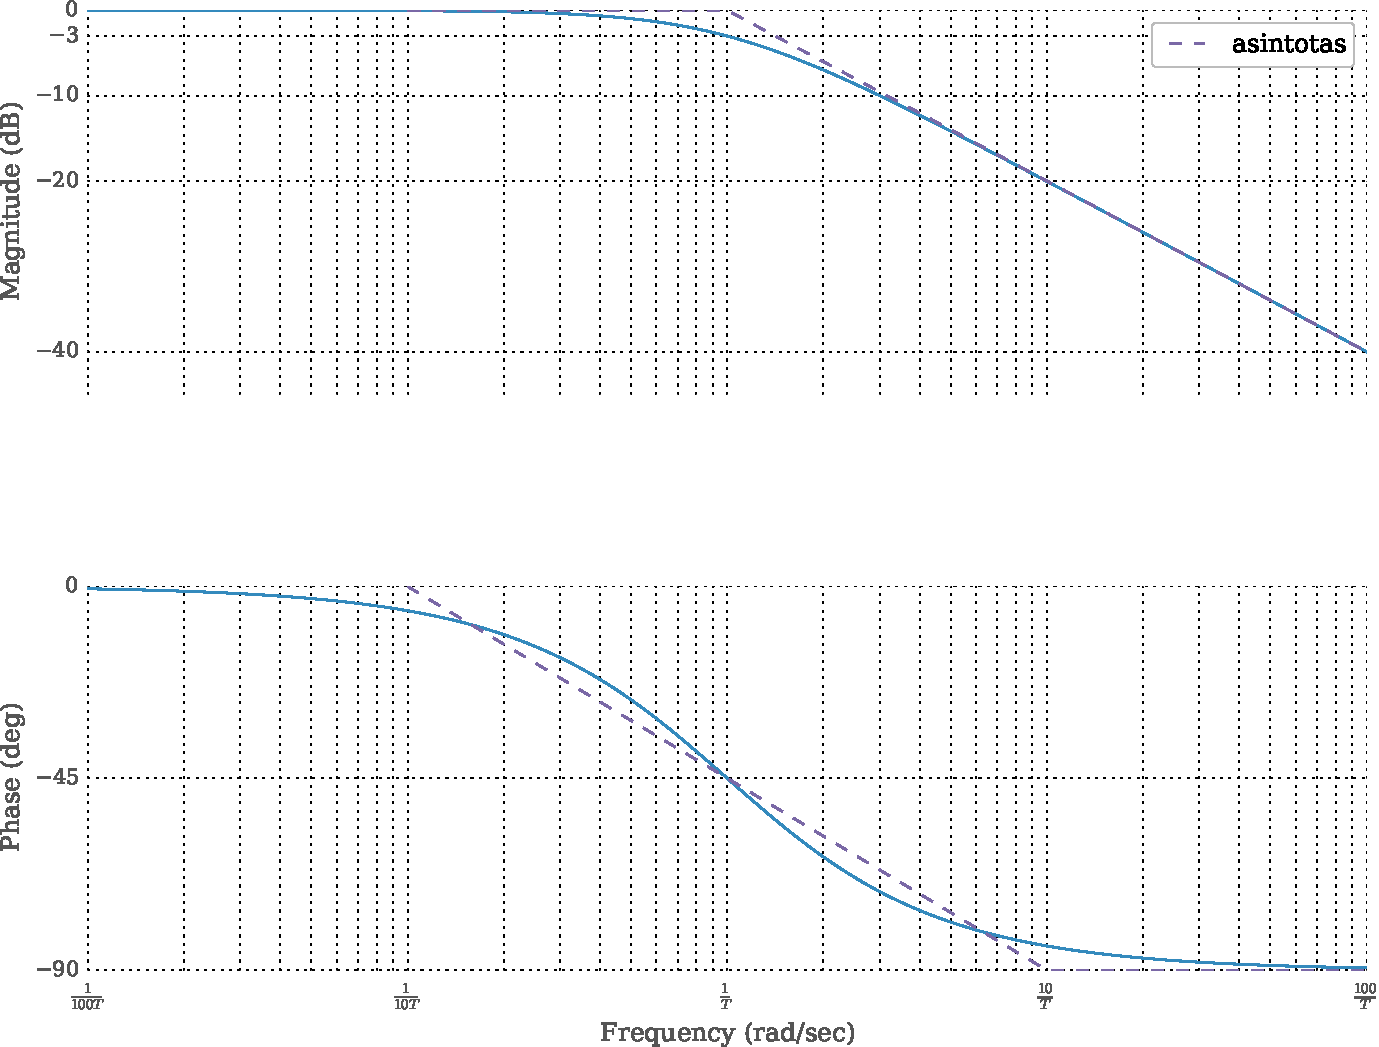
\includegraphics[width=0.5\textwidth]{./imagenes/bodeprimerorden.pdf}
            \caption{\label{fig:bodeprimerorden}Diagrama de Bode del sistema $G(s) = \frac{1}{Ts + 1}$.}
        \end{figure}

        De manera similar podemos gráficar el sistema inverso $G(s) =Ts + 1$ en la figura~\ref{fig:bodeprimerordeninverso}.

        \begin{figure}
            \centering
            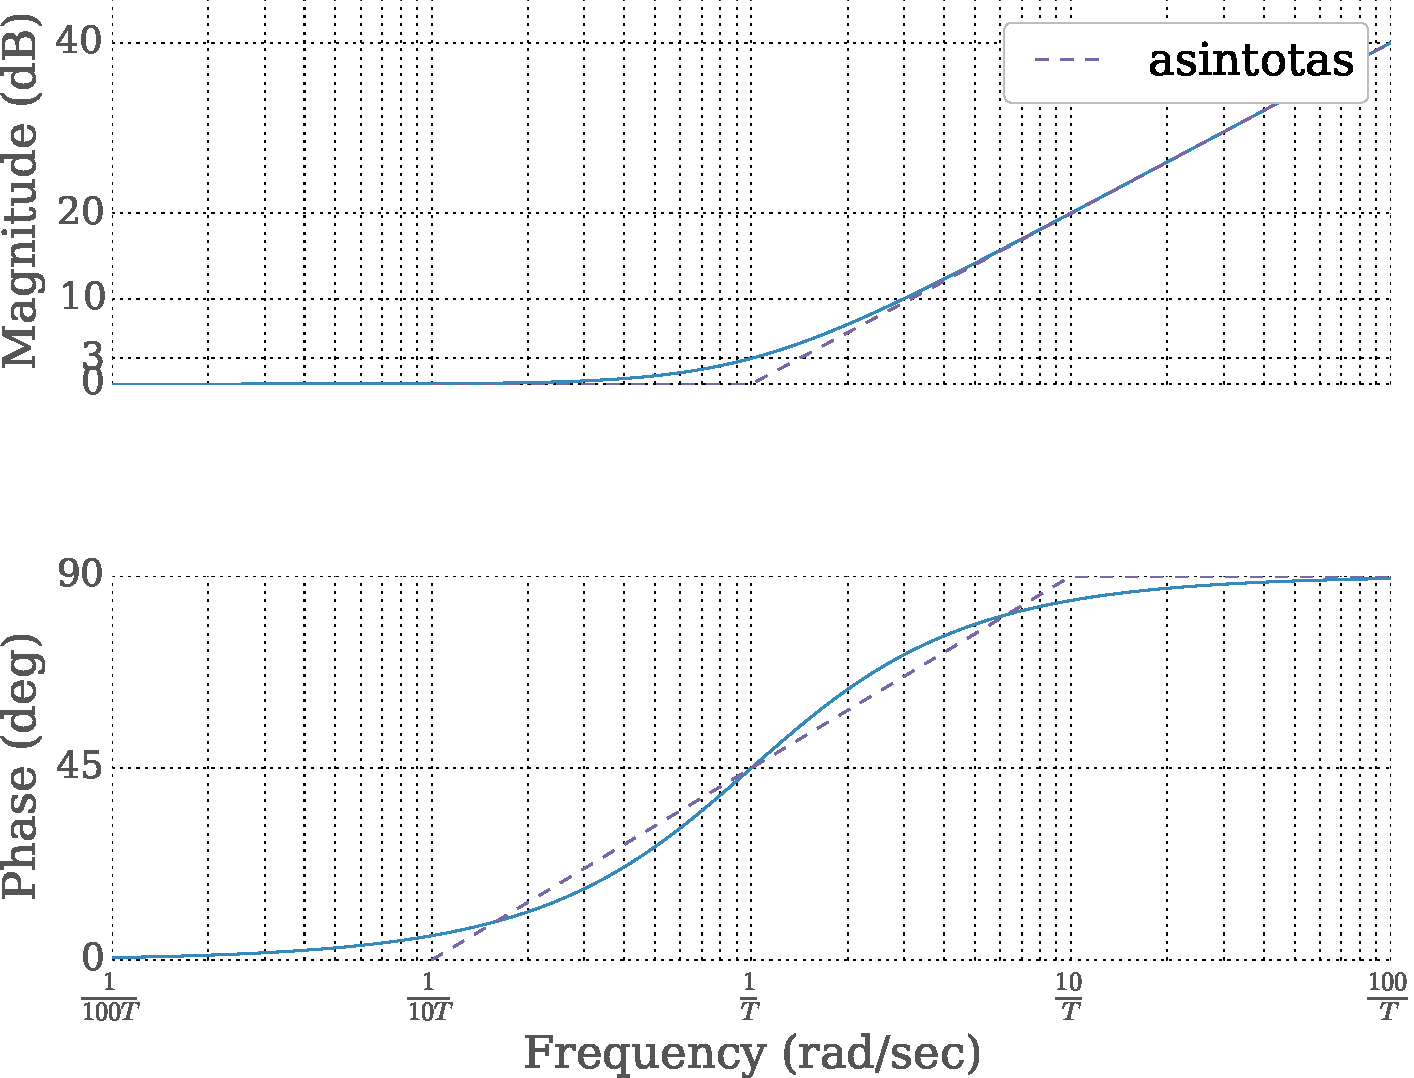
\includegraphics[width=0.5\textwidth]{./imagenes/bodeprimerordeninverso.pdf}
            \caption{\label{fig:bodeprimerordeninverso}Diagrama de Bode del sistema $G(s) = Ts + 1$.}
        \end{figure}

        \subsection{Factor integral}

            Dado el sistema $G(s) = \frac{1}{s}$ tendremos los siguientes valores para la magnitud y la fase:

            \begin{eqnarray*}
                \left| G(j \omega) \right|_{dB} & = & \left| \frac{1}{j \omega} \right|_{dB} = -20 \log{(\omega)} \\
                \phase{G(j \omega)} & = & -90^o
            \end{eqnarray*}

            Por lo que el diagrama de Bode queda como en la figura~\ref{fig:bodeintegral}.

            \begin{figure}
                \centering
                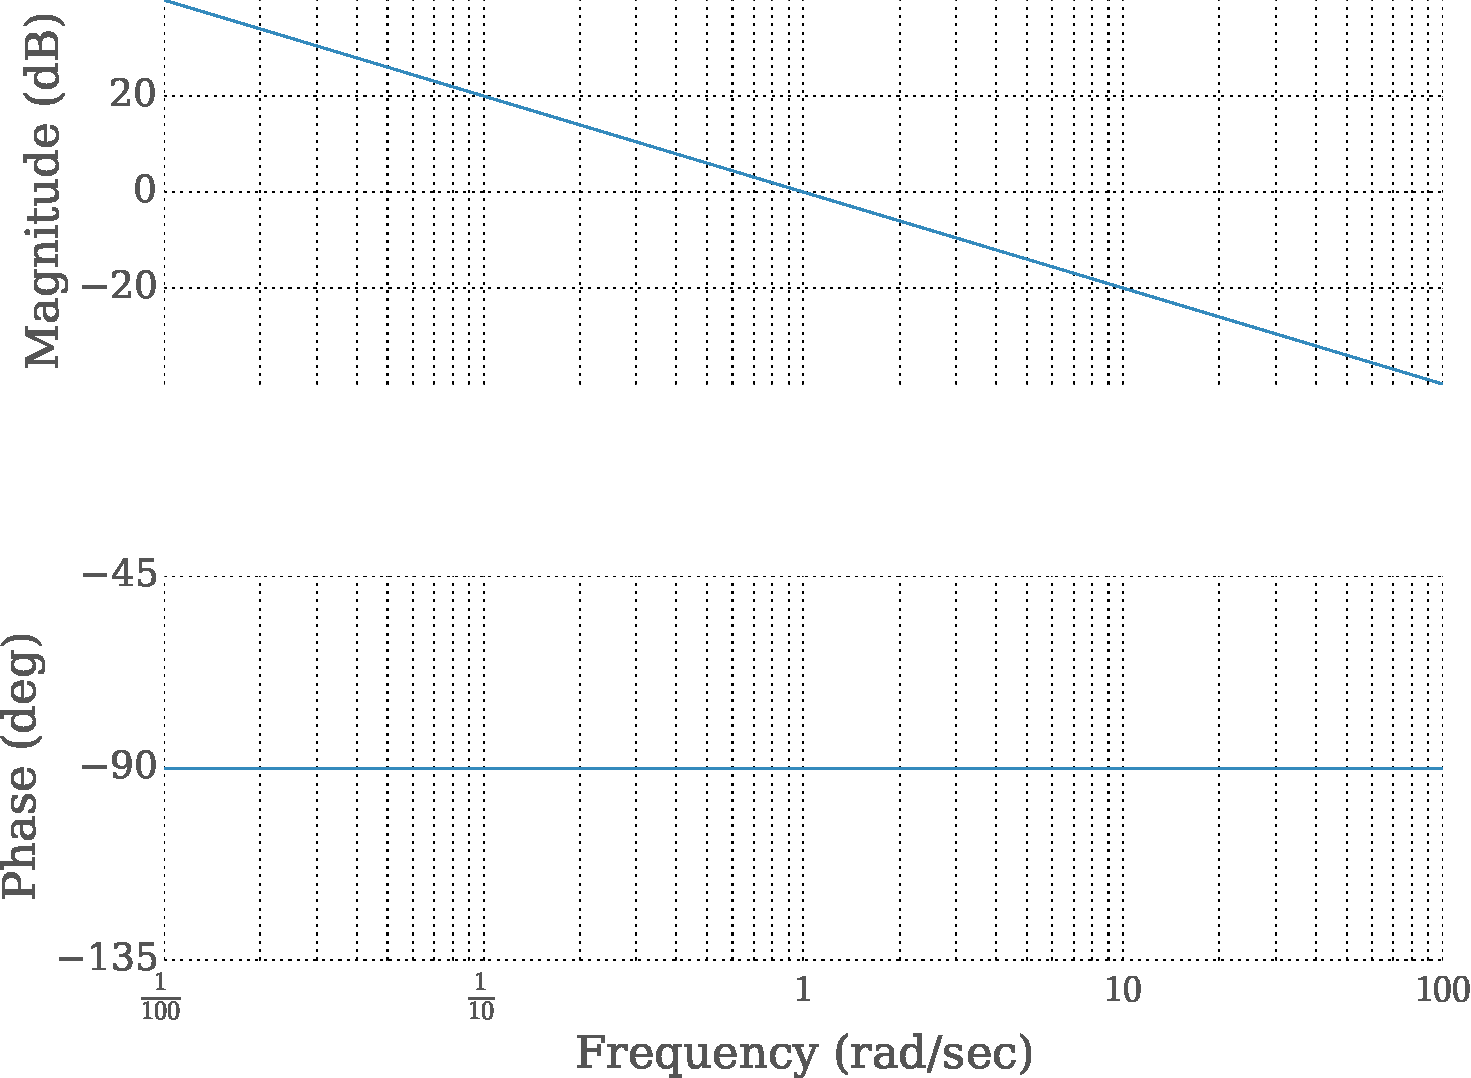
\includegraphics[width=0.5\textwidth]{./imagenes/bodeintegral.pdf}
                \caption{\label{fig:bodeintegral}Diagrama de Bode del sistema $G(s) = \frac{1}{s}$.}
            \end{figure}

        \subsection{Factor derivativo}

            Dado el sistema $G(s) = s$ tendremos los siguientes valores para la magnitud y la fase:

            \begin{eqnarray*}
                \left| G(j \omega) \right|_{dB} & = & \left| j \omega \right|_{dB} = 20 \log{(\omega)} \\
                \phase{G(j \omega)} & = & 90^o
            \end{eqnarray*}

            Por lo que el diagrama de Bode queda como en la figura~\ref{fig:bodederivativo}.

            \begin{figure}
                \centering
                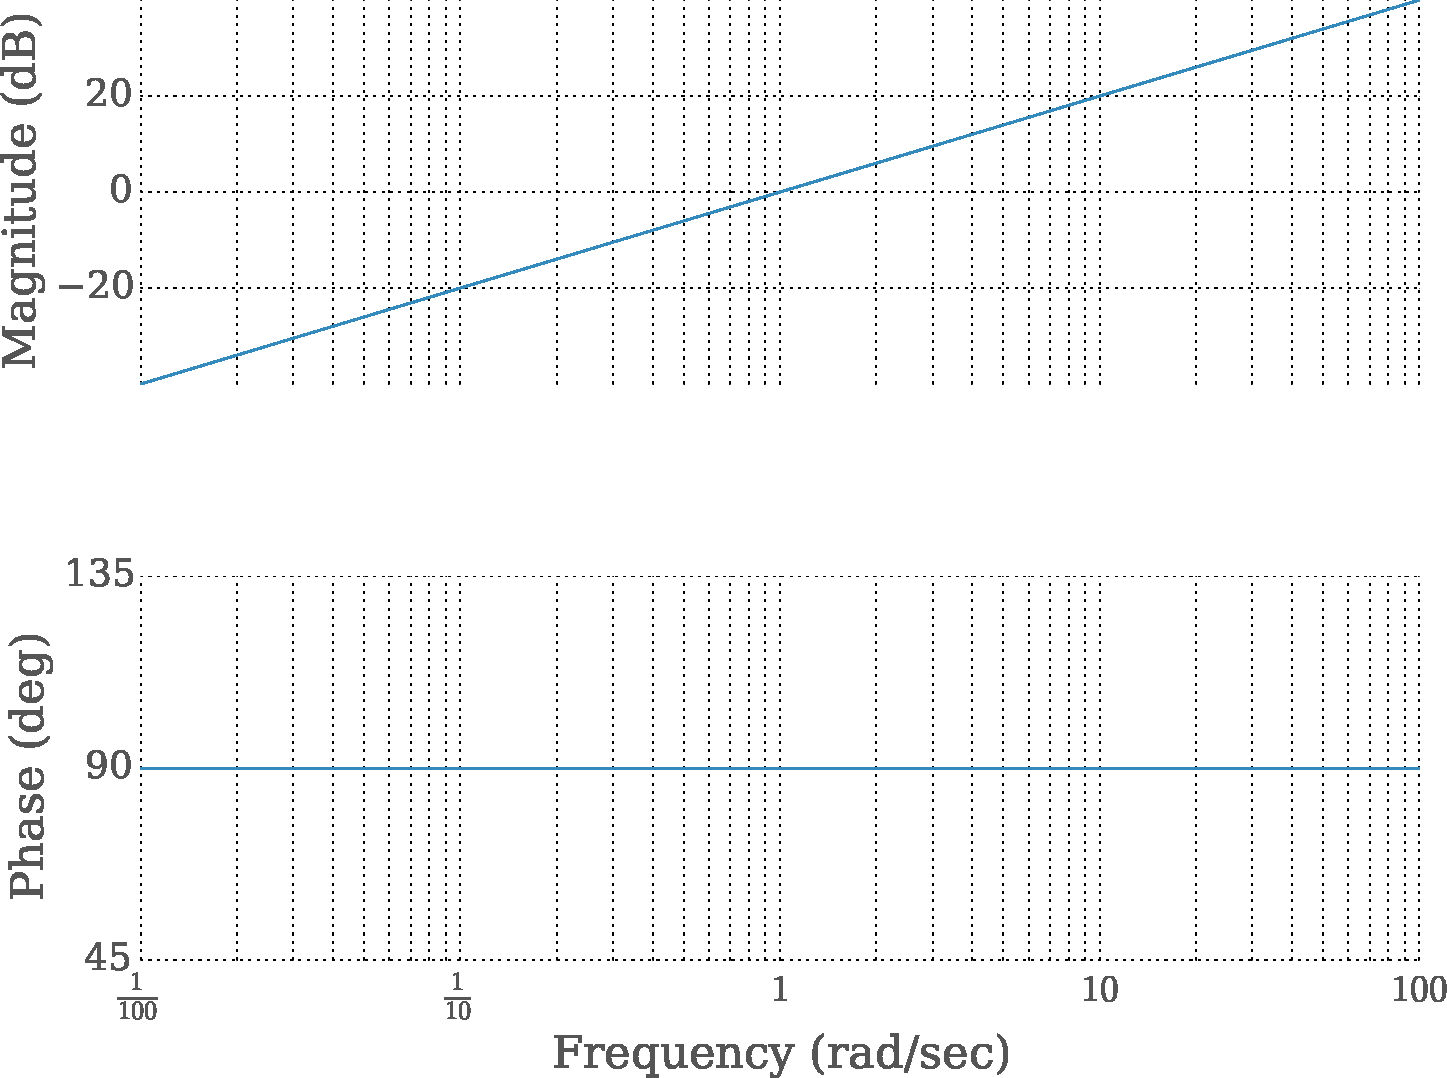
\includegraphics[width=0.5\textwidth]{./imagenes/bodederivativo.pdf}
                \caption{\label{fig:bodederivativo}Diagrama de Bode del sistema $G(s) = s$.}
            \end{figure}

    \newpage
    \section{Factores de segundo orden}

        Dado el sistema de segundo orden

        \begin{equation*}
            G(s) = \frac{1}{\left( \frac{s}{\omega_n} \right)^2 + 2 \zeta \left( \frac{s}{\omega_n} \right) + 1}
        \end{equation*}

        tendremos que su magnitud y fase estarán dados por:

        \begin{eqnarray*}
            \left| G(j \omega) \right|_{dB} & = & -20 \log{\sqrt{\left( 1 - \left( \frac{\omega}{\omega_n} \right)^2 \right)^2 + \left( 2 \zeta \left( \frac{\omega}{\omega_n} \right) \right)^2}} \\
            \phase{G(j \omega)} & = & -\arctan{\left( \frac{2 \zeta \left( \frac{\omega}{\omega_n} \right)}{1 - \left( \frac{\omega}{\omega_n} \right)^2} \right)}
        \end{eqnarray*}

        De estas ecuaciones, podemos aproximar su comportamiento cuando $\frac{\omega}{\omega_n}$ es muy grande o muy pequeño:

        \begin{eqnarray*}
            \frac{\omega}{\omega_n} \ll 1 & \implies & \left| G(j \omega) \right|_{dB} \approx -20 \log{\sqrt{1}} = 0 dB \\
            \frac{\omega}{\omega_n} \gg 1 & \implies & \left| G(j \omega) \right|_{dB} \approx -20 \log{\sqrt{\left( \frac{\omega}{\omega_n} \right)^4}} = -40 \log{\left( \frac{\omega}{\omega_n} \right)} dB
        \end{eqnarray*}

        \subsection{Frecuencia de resonancia $\omega_r$}

            Para encontrar la frecuencia de resonancia, necesitamos encontrar el punto en que la gráfica de magnitud cambia de dirección, es decir cuando la derivada cambia de signo. Por comodidad lo haremos con la función auxiliar $g(s) = \left( 1 - \left( \frac{\omega}{\omega_n} \right)^2 + \left( 2 \zeta \left( \frac{\omega}{\omega_n} \right) \right)^2 \right)$. Asi pues, la derivada será:

            \begin{eqnarray*}
                \frac{d g}{d \omega} & = & 2 \left( 1 - \left( \frac{\omega}{\omega_n} \right)^2 \right) \left( -2 \frac{\omega}{\omega_n} \right) + 4 \zeta^2 (2) \left( \frac{\omega}{\omega_n} \right) \\
                & = & -4 \frac{\omega}{\omega_n} \left( 1 - \left( \frac{\omega}{\omega_n} \right)^2 \right) + 4 \frac{\omega}{\omega_n} \left( 2 \zeta^2 \right) \\
                & = & 4 \frac{\omega}{\omega_n} \left( \left( \frac{\omega}{\omega_n} \right)^2 - 1 + 2 \zeta^2 \right) = 0
            \end{eqnarray*}

            por lo que la gráfica tiene pendiente nula cuando $\omega = 0$ o bien cuando $\left( \frac{\omega}{\omega_n} \right)^2 - 1 + 2 \zeta^2 = 0$, por lo que podemos ver que la frecuencia de resonancia se encuentra cuando:

            \begin{eqnarray*}
                \left( \frac{\omega}{\omega_n} \right)^2 & = & 1 - 2 \zeta^2 \\
                \frac{\omega}{\omega_n} & = & \sqrt{1 - 2 \zeta^2} \\
                \omega_r & = & \omega_n \sqrt{1 - 2 \zeta^2}
            \end{eqnarray*}

            donde $0 \le \zeta \le \frac{1}{\sqrt{2}}$.

        \subsection{Valor pico de resonancia $M_R$}

            Si sustituimos esta frecuencia de resonancia en la magnitud, tendremos el valor pico de resonancia.

    \newpage
    \section{Factores de orden cero}
        \faltante{Falta escribir apunte}


    \clearpage
    
\section{Diagramas de Nyquist}
    \subsection{Factor integral}
    \subsection{Factor derivativo}
    \subsection{Factores de primer orden}
    \subsection{Factores de segundo orden}


    \clearpage
    %-------------------------------------------------------------------------------
%	EMPIEZA CAPITULO
%-------------------------------------------------------------------------------

\chapter{Criterio de Estabilidad de Nyquist}

%-------------------------------------------------------------------------------
%	EMPIEZA SECCION
%-------------------------------------------------------------------------------

    \section{Ejemplos}
    \faltante{Falta escribir apunte}


    \clearpage
    
\chapter{Estabilidad Relativa}
    \section{Margen de Fase}
        \subsection{Estable}
        \subsection{Inestable}
    \section{Margen de Ganancia}
        \subsection{Estable}
        \subsection{Inestable}


    \clearpage
    
\chapter{Compensador de adelanto y atrase de fase (Frecuencia)}
    \section{Compensador de adelanto de fase}
    \section{Compensador de atraso de fase}
    \section{Ejemplos}


    \clearpage
    
\section{Controladores PID}
    \subsection{Sintonización: Reglas de Ziegler-Nichols}
        \subsubsection{Respuesta al escalón}
        \subsubsection{Respuesta a oscilaciones sostenidas}
    \subsection{Esquemas modificados}
        \subsubsection{Controlador PID}
        \subsubsection{Controlador PI-D}
        \subsubsection{Controlador I-PD}


    \clearpage
    
\chapter{Representación de estado}

    La siguiente funcion de transferencia es la Transformada de Laplace de la ecuacion diferencial ordinaria de orden $n$ que describe al sistema.

    \begin{equation}
        \frac{\hat{y}(s)}{\hat{u}(s)} = \frac{b_0 s^m + b_1 s^{m-1} + ... + b_{m-1} s + b_m}{s^n + a_1 s^{n-1} + ... + a_{n-1} s + a_n} = \frac{B(s)}{A(s)}, m \le n
    \end{equation}

    \begin{multline}
        \frac{d^n}{dt^n} y(t) + a_1 \frac{d^{n-1}}{dt^{n-1}} y(t) + \dots + a_{n-1} \frac{d}{dt} y(t) + a_n \frac{d}{dt} y(t) \\ = b_0 \frac{d^m}{dt^m} u(t) + b_1 \frac{d^{m-1}{dt^{m-1}}} u(t) + \dots + b_{m-1} \frac{d}{dt} u(t) + b_{m} u(t)
    \end{multline}

    Haciendo la siguiente asignacion de variables:

    \begin{eqnarray}
    x_1     & = & z \nonumber \\
    x_2     & = & \frac{d}{dt} x_1 = \frac{d}{dt} z \nonumber \\
    x_3     & = & \frac{d}{dt} x_2 = \frac{d^2}{dt^2} z \nonumber \\
    \vdots  & = & \vdots \nonumber \\
    x_{n-1} & = & \frac{d}{dt} x_{n-2} = \frac{d^{n-2}}{dt^{n-2}} z \nonumber \\
    x_n     & = & \frac{d}{dt} x_{n-1} = \frac{d^{n-1}}{d^{n-1}} z \nonumber
    \end{eqnarray}

    Donde:

    \begin{equation}
        \frac{d}{dt} x_n = -a_n x_1 - a_{n-1} x_2 - \dots - a_2 x_{n-1} - a_1 x_n + u(t)
    \end{equation}
    \begin{equation}
        y = b_m x_1 + b_{m-1} x_2 + \dots + b_1 x_{m-1} + b_0 x_m
    \end{equation}

    Por lo que se obtiene:

    \begin{math}
        \left( \frac{d^n}{dt^n} + a_1 \frac{d^{n-1}}{dt^{n-1}} + \dots + a_{n-1} \frac{d}{dt} + a_n \right) z(t) = u(t)
    \end{math}

    \begin{math}
        y(t) = \left( b_m + b_{m-1} \frac{d}{dt} + \dots + b_1 \frac{d^{m-1}}{dt^{m-1}} + b_0 \frac{d^m}{dt^m} \right) z(t)
    \end{math}

    es decir:

    \begin{equation}
        M \left( \frac{d}{dt} \right) z(t) = u(t)
    \end{equation}

    \begin{equation}
        y(t) = N \left( \frac{d}{dt} \right) z(t)
    \end{equation}

    Lo cual implica $M \left( \frac{d}{dt} \right) y(t) = N \left( \frac{d}{dt} \right) u(t)$. Donde:

    \begin{math}
        M \left( \frac{d}{dt} \right) = \left( \frac{d^n}{dt^n} + a_1 \frac{d^{n-1}}{dt^{n-1}} + \dots + a_{n-1} \frac{d}{dt} + a_n \right)
    \end{math}

    \begin{math}
        N \left( \frac{d}{dt} \right) = \left( b_m + b_{m-1} \frac{d}{dt} + \dots + b_1 \frac{d^{m-1}}{dt^{m-1}} + b_0 \frac{d^m}{dt^m} \right)
    \end{math}

    Esta es la misma ecuación diferencial con la que empezamos. Note que la escritura matricial de esta Ecuación Diferencial Ordinaria es:

    \begin{equation}
        \frac{d}{dt} \vec{x} = A \vec{x}(t) + \vec{b} u(t)
    \end{equation}

    \begin{equation}
        \vec{y}(t) = \vec{c} \cdot \vec{x}(t)
    \end{equation}

    Donde:

    \begin{equation}
        \vec{x}(t) =
        \begin{pmatrix}
        x_1(t) \\
        x_2(t) \\
        \vdots \\
        x_n(t)
        \end{pmatrix}
    \end{equation}

    \begin{equation}
        A =
        \begin{pmatrix}
        0 & 1 & 0 & \dots & 0 & 0 \\
        0 & 0 & 1 & \dots & 0 & 0 \\
        0 & 0 & 0 & \dots & 0 & 0 \\
        \vdots & \vdots & \vdots &   & \vdots & \vdots \\
        0 & 0 & 0 & \dots & 0 & 1 \\
        -a_n & -a_{n-1} & -a_{n-2} & \dots & -a_2 & -a_1
        \end{pmatrix}
    \end{equation}

    \begin{equation}
        \vec{b} =
        \begin{pmatrix}
        0 \\
        0 \\
        \vdots \\
        1
        \end{pmatrix}
    \end{equation}

    \begin{equation}
        \vec{c} =
        \begin{pmatrix}
        b_m     \\
        b_{m-1} \\
        \vdots  \\
        b_1     \\
        b_0     \\
        \vdots  \\
        0       \\
        0
        \end{pmatrix}
    \end{equation}

    \begin{center}
        \tikzstyle{input} = [coordinate]
        \tikzstyle{output} = [coordinate]
        \tikzstyle{empty} = [coordinate]
        \tikzstyle{block} = [draw, rectangle, minimum height=2.25em, minimum width=2.25em]
        \tikzstyle{sum} = [draw, circle]
        \tikzstyle{init} = [pin edge={to-, thin, black}]

        \begin{tikzpicture}[auto, node distance=1.1cm, >=latex']
            \node [input, name=entrada] {};
            \node [sum, right of=entrada] (s1) {$+$};
            \node [block, right of=s1] (int1) {$\int$};
            \node [inner sep=0,minimum size=0,right of=int1] (xn) {};
            \node [block, right of=xn] (int2) {$\int$};
            \node [inner sep=0,minimum size=0,right of=int2] (xn1) {};
            \node [block, draw=none, right of=xn1] (vacio) {$\dots$};
            \node [inner sep=0,minimum size=0,right of=vacio] (x3) {};
            \node [block, right of=x3] (int3) {$\int$};
            \node [inner sep=0,minimum size=0,right of=int3] (x2) {};
            \node [block, right of=x2] (int4) {$\int$};
            \node [inner sep=0,minimum size=0,right of=int4] (x1) {};
            \node [block, right of=x1] (bm) {$b_m$};
            \node [sum, right of=bm] (s2) {$+$};
            \node [output, right of=s2] (salida) {};

            \node [block, below of=int1] (a1) {$-a_1$};
            \node [block, below of=a1] (a2) {$-a_2$};
            \node [block, draw=none, below of=a2] (avacio) {$\vdots$};
            \node [block, below of=avacio] (an1) {$-a_{n-1}$};
            \node [block, below of=an1] (an) {$-a_n$};

            \node [block, above of=bm] (bm1) {$b_{m-1}$};
            \node [block, draw=none, above of=bm1] (bvacio) {$\vdots$};
            \node [block, above of=bvacio] (b1) {$b_{1}$};
            \node [block, above of=b1] (b0) {$b_{0}$};

            \draw [->] (entrada) -- node[name=u] {$u(t)$} (s1);
            \draw [->] (s1)      -- (int1);
            \draw [->] (int1)    -- node[name=xn] {$x_n$} (int2);
            \draw [->] (int2)    -- node[name=xn1] {$x_{n-1}$} (vacio);
            \draw [->] (vacio)   -- node[name=x3] {$x_3$} (int3);
            \draw [->] (int3)    -- node[name=x2] {$x_2$} (int4);
            \draw [->] (int4)    -- node[name=x1] {$x_1$} (bm);
            \draw [->] (bm)      -- (s2);
            \draw [->] (s2)      -- node[name=y] {$y(t)$} (salida);

            \draw [->] (xn)  |- (a1);
            \draw [->] (xn1) |- (a2);
            \draw [->] (x2)  |- (an1);
            \draw [->] (x1)  |- (an);

            \draw [->] (a1)  -| (s1.324);
            \draw [->] (a2)  -| (s1.288);
            \draw [->] (an1) -| (s1.252);
            \draw [->] (an)  -| (s1.216);

            \draw [->] (xn)  |- (b0);
            \draw [->] (xn1) |- (b1);
            \draw [->] (x2)  |- (bm1);

            \draw [->] (b0)  -| (s2.45);
            \draw [->] (b1)  -| (s2.90);
            \draw [->] (bm1) -| (s2.135);
        \end{tikzpicture}
    \end{center}

    \section{Solución temporal de la ecuación de estado}

    \begin{enumerate}

    \item Para el caso en que $A$ es un escalar y la solución es homogénea se considera la siguiente Ecuación Diferencial Ordinaria:

        \begin{equation}
            \frac{d}{dt} x(t) = a x(t) \mid x(0) = x_0
        \end{equation}

        Suponga una solución de la forma:

        \begin{equation}
            x(t) = \alpha_0 + \alpha_1 t + \alpha_2 t^2 + \dots + \alpha_k t^k + \dots
        \end{equation}

        Entonces se tiene:

        \begin{multline}
            \alpha_1 + 2 \alpha_2 t + 3 \alpha_3 t^2 + \dots + k \alpha_k t^{k-1} + \dots \\ = a \alpha_0 + a \alpha_1 t + a \alpha_2 t^2 + \dots + a \alpha_k t^k + \dots \nonumber
        \end{multline}

        Por lo que las $\alpha_i$ deben satisfacer:

        \begin{equation}
            \begin{array}{c c c c c}
            \alpha_1 & = & a \alpha_0     & = & \frac{1}{1!} a^1 \alpha_0 \\
            \alpha_2 & = & a \alpha_1     & = & \frac{1}{2!} a^2 \alpha_0 \\
            \alpha_3 & = & a \alpha_2     & = & \frac{1}{3!} a^3 \alpha_0 \\
            \vdots   & = & \vdots         & = & \vdots                    \\
            \alpha_k & = & a \alpha_{k-1} & = & \frac{1}{k!} a^k \alpha_0 \\
            \end{array} \quad ; \quad \alpha_0 = x_0
        \end{equation}

        Esto es:

        \begin{equation}
            x(t) = \left( \sum\limits_{i = 0}^{\infty} \frac{1}{i!} (a t)^i \right) x_0 \nonumber
        \end{equation}

        \begin{equation}
            x(t) = e^{at} x_0
        \end{equation}

        Notese que: $\frac{d}{dt} x(t) = \left( \sum\limits_{i=0}^{\infty} \frac{1}{i!} \frac{d}{dt} (at)^i \right) x_0 = \left( \sum\limits_{i=1}^{\infty} \frac{1}{(i-1)!} (at)^{i-1} \right) a x_0 = \left( \sum\limits_{j=0}^{\infty} \frac{1}{j!} (at)^j \right) a x_0$

        \begin{math}
            \frac{d}{dt} x(t) = a e^{at} x_0 = a x(t) \quad x(0) = x_0
        \end{math}

    \item Para el caso en que $A$ es una matriz y la solución es homogénea se considera la siguiente Ecuación Diferencial Ordinaria:

        \begin{equation}
            \frac{d}{dt} \vec{x}(t) = a \vec{x}(t) \mid \vec{x}(0) = \vec{x}_0
        \end{equation}

        De la misma manera que en el caso escalar, se supone una solución de la forma:

        \begin{equation}
            \vec{x}(t) = \vec{\alpha}_0 + \vec{\alpha}_1 t + \vec{\alpha}_2 t^2 + \dots + \vec{\alpha}_k t^k + \dots
        \end{equation}

        Entonces se tiene:

        \begin{multline}
            \vec{\alpha}_1 + 2 \vec{\alpha}_2 t + 3 \vec{\alpha}_3 t^2 + \dots + k \vec{\alpha}_k t^{k-1} + \dots \\ = A \vec{\alpha}_0 + A \vec{\alpha}_1 t + A \vec{\alpha}_2 t^2 + \dots + A \vec{\alpha}_k t^k + \dots \nonumber
        \end{multline}

        Por lo que las $\vec{\alpha}_i$ deben satisfacer:

        \begin{equation}
            \begin{array}{c c c c c}
            \vec{\alpha}_1 & = & A \vec{\alpha}_0     & = & \frac{1}{1!} A^1 \vec{\alpha}_0 \\
            \vec{\alpha}_2 & = & A \vec{\alpha}_1     & = & \frac{1}{2!} A^2 \vec{\alpha}_0 \\
            \vec{\alpha}_3 & = & A \vec{\alpha}_2     & = & \frac{1}{3!} A^3 \vec{\alpha}_0 \\
            \vdots   & = & \vdots         & = & \vdots                    \\
            \vec{\alpha}_k & = & A \vec{\alpha}_{k-1} & = & \frac{1}{k!} A^k \vec{\alpha}_0 \\
            \end{array} \quad ; \quad \vec{\alpha}_0 = \vec{x}_0
        \end{equation}

        Esto es:

        \begin{equation}
            \vec{x}(t) = \left( \sum\limits_{i = 0}^{\infty} \frac{1}{i!} (A t)^i \right) \vec{x}_0 \nonumber
        \end{equation}

        En análisis real, se demuestra que esta serie es absolutamente convergente y se define como:

        \begin{equation}
            \exp{(At)} = \sum\limits_{i = 0}^{\infty} \frac{1}{i!} (A t)^i
        \end{equation}

        Notese que:

        \begin{math}
            \frac{d}{dt} \exp{(At)} = \frac{d}{dt} \sum\limits_{i=0}^{\infty} \frac{1}{i!} (At)^i = \left( \sum\limits_{i=1}^{\infty} \frac{1}{(i-1)!} (At)^{i-1} \right) A = A \sum\limits_{j=0}^{\infty} \frac{1}{j!} (At)^j = A \exp{(At)}
        \end{math}

        Por lo que:

        \begin{math}
            \vec{x}(t) = \exp{(At)} \vec{x}_0
        \end{math}

        \begin{math}
            \frac{d}{dt} \vec{x}(t) = A \exp{(At)} \vec{x}_0 = A \vec{x}(t) \quad \vec{x}(0) = \vec{x}_0
        \end{math}

    \item Para el caso en que $A$ es escalar y la solución es forzada:

        \begin{equation}
            \frac{d}{dt} x(t) = a x(t) + b u(t) \mid x(0) = 0
        \end{equation}

        La solución a esta ecuación es:

        \begin{equation}
            x(t) = \int_0^t e^{a(t-\tau)} b u(\tau) \, d \tau
        \end{equation}

        \begin{math}
            \frac{d}{dt} x(t) = e^{a(t-t)} b u(t) + \int_0^t \frac{d}{dt} e^{a(t-\tau)} b u(\tau) \, d \tau = b u(t) + a \int_0^t e^{a(t-\tau)} b u(\tau) \, d \tau
        \end{math}

        \begin{equation}
            \frac{d}{dt} x(t) = b u(t) + a x(t)
        \end{equation}

        Por lo que la solución general (con $x(0) = x_0$):

        \begin{equation}
            x(t) = e^{at} x_0 + \int_0^t e^{a(t-\tau)} b u(\tau) \, d \tau
        \end{equation}

    \item Para el caso en que $A$ es una matriz y la solución es forzada:

        \begin{equation}
            \frac{d}{dt} \vec{x}(t) = A \vec{x}(t) + \vec{b} u(t) \mid \vec{x}(0) = 0
        \end{equation}

        La solución de esta ecuación es:

        \begin{equation}
            \vec{x}(t) = \int_0^t \exp{(A(t-\tau))} \vec{b} u(\tau) \, d \tau
        \end{equation}

        En efecto, derivando tenemos:

        \begin{math}
            \frac{d}{dt} \vec{x}(t) = \exp{(A(t-t))} \vec{b} u(t) + \int_0^t \frac{d}{dt} \exp{(A(t-\tau))} \vec{b} u(\tau) \, d \tau = \vec{b} u(t) + A \int_0^t \exp{(A(t-\tau))} \vec{b} u(\tau) \, d \tau
        \end{math}

        \begin{equation}
            \frac{d}{dt} \vec{x}(t) = \vec{b} u(t) + a \vec{x}(t)
        \end{equation}

        Por lo que la solución general (con $x(0) = x_0$):

        \begin{equation}
            \vec{x}(t) = \exp{(At)} \vec{x}_0 + \int_0^t \exp{(A(t-\tau))} \vec{b} u(\tau) \, d \tau
        \end{equation}

    \end{enumerate}

    \section{Función (Matriz) de transferencia de la ecuación de estado}

        \begin{enumerate}

        \item
        Para el caso escalar, se tiene que la transformada de Laplace con coeficientes independientes nulos es:

        \begin{align}
        s x(s)       & = a x(s) + b u(s) \nonumber\\
        (s - a) x(s) & = b u(s) \nonumber\\
        x(s)         & = (s - a)^{-1} b u(s) \nonumber\\
        x(s)         & = \frac{b}{s - a} u(s) \nonumber
        \end{align}

        Por lo que:

        \begin{equation}
        e^{at} = \mathcal{L}^{-1} \left\{ (s - a)^{-1} \right\}
        \end{equation}

        \item
        Para el caso matricial, tenemos que la transformada de Laplace con coeficientes independientes nulos es:

        \begin{align}
        s \vec{x}(s)         & = A \vec{x}(s) + \vec{b} u(s) \nonumber \\
        (s I - A) \vec{x}(s) & = \vec{b} u(s) \nonumber \\
        x(s)                 & = (s I - A)^{-1} \vec{b} u(s) \nonumber
        \end{align}

        Por lo que:

        \begin{equation}
        \exp{(At)} = \mathcal{L}^{-1} \left\{ (s I - A)^{-1} \right\}
        \end{equation}

        \end{enumerate}

    \section{Función de transferencia de la representación de estado}

        Sea la siguiente Ecuación Diferencial Ordinaria:

        \begin{equation}
            M \left( \frac{d}{dt} \right) y(t) = N \left( \frac{d}{dt} \right) u(t) \nonumber
        \end{equation}

        donde:

        \begin{math}
            M \left( \frac{d}{dt} \right) = \frac{d^n}{dt^n} + a_1 \frac{d^{n-1}}{dt^{n-1}} + \dots + a_{n-1} \frac{d}{dt} + a_n
        \end{math}

        \begin{math}
            N \left( \frac{d}{dt} \right) = b_m + b_{m-1} \frac{d}{dt} + \dots + b_1 \frac{d^{m-1}}{dt^{m-1}} + b_0 \frac{d^m}{dt^m}
        \end{math}

        La función de transferencia con coeficientes independientes nulos de las ecuaciones es:

        \begin{equation}
            F(s) = \frac{N(s)}{M(s)} = \frac{\frac{d^n}{dt^n} + a_1 \frac{d^{n-1}}{dt^{n-1}} + \dots + a_{n-1} \frac{d}{dt} + a_n}{b_m + b_{m-1} \frac{d}{dt} + \dots + b_1 \frac{d^{m-1}}{dt^{m-1}} + b_0 \frac{d^m}{dt^m}}
        \end{equation}

        \begin{description}
            \item [Ceros.] Las raíces del polinomio $N(s)$.
            \item [Polos.] Las raíces del polinomio $M(s)$.
        \end{description}

        Sea la siguiente representación de estado de la Ecuación Diferencial Ordinaria:

        \begin{eqnarray}
        \frac{d}{dt} x & = & A x + b u \nonumber \\
        y & = & c x + d u \nonumber
        \end{eqnarray}

        La función de transferencia con coeficientes independientes nulos en esta representación es:

        \begin{eqnarray}
        s x(s) & = & A x(s) + b u(s) \nonumber \\
        y(s) & = & c x(s) + d u(s) \nonumber
        \end{eqnarray}

        \begin{equation}
            \vdots \nonumber
        \end{equation}

        \begin{eqnarray}
        (s I - A) x(s) & = & b u(s) \nonumber \\
        y(s) & = & c x(s) + d u(s) \nonumber
        \end{eqnarray}

        \begin{equation}
            \vdots \nonumber
        \end{equation}

        \begin{eqnarray}
        x(s) & = & (s I - A)^{-1} b u(s) \nonumber \\
        y(s) & = & c x(s) + d u(s) \nonumber
        \end{eqnarray}

        \begin{equation}
            \vdots \nonumber
        \end{equation}

        \begin{equation}
            y(s) = c[(s I - A)^{-1} b u(s)] + d u(s) = [c(s I - A)^{-1} b + d] u(s) \nonumber
        \end{equation}

        \begin{equation}
            \vdots \nonumber
        \end{equation}

        \begin{equation}
            F(s) = c(s I - A)^{-1} b + d
        \end{equation}

    \section{Matriz sistema}

        \begin{equation}
            \Sigma(s) =
            \begin{pmatrix}
            sI - A & b \\
            -c & d
            \end{pmatrix}
        \end{equation}

        Note que:

        \begin{multline}
            \begin{pmatrix}
            (sI - A)^{-1} & 0 \\
            0 & I
            \end{pmatrix}
            \begin{pmatrix}
            sI - A & b \\
            -c & d
            \end{pmatrix}
            \begin{pmatrix}
            I & -(sI - A)b \\
            0 & I
            \end{pmatrix}
            \\
            =
            \begin{pmatrix}
            I & (sI - A)^{-1} b \\
            -c & d
            \end{pmatrix}
            \begin{pmatrix}
            I & -(sI - A)b \\
            0 & I
            \end{pmatrix}
            \\
            =
            \begin{pmatrix}
            I & 0 \\
            -c & (c(sI - A)^{-1} b + d)
            \end{pmatrix}
            \nonumber
        \end{multline}

        Por lo que:

        \begin{math}
            \det{\left( (sI - A)^{-1} \right)} \cdot \det{\left( \Sigma(s) \right)} \cdot I = c(sI - A)^{-1} b + d
        \end{math}

        \begin{equation}
            F(s) = \frac{\det{\left( \Sigma(s) \right)}}{\det{\left( sI - A \right)}}
        \end{equation}

        Por lo que los polos coinciden con los valores propios de $A$ y los ceros son los números complejos que hacen perder rango a la matriz sistema.

        \begin{equation}
            \text{Polos: } F(s) = \left\{ s \in \mathbbm{C} \mid \det{\left( sI - A \right)} = 0 \right\}
        \end{equation}

        \begin{equation}
            \text{Ceros: } F(s) = \left\{ s \in \mathbbm{C} \mid \det{\left( \Sigma(s) \right)} = 0 \right\}
        \end{equation}

    \section{Propiedades de la Matriz A}
        \begin{enumerate}[i)]
            \item
            \begin{equation}
                \exp{(A t)} = \sum\limits_{i=0}^{\infty} \frac{1}{i!} (A t)^i
            \end{equation}

            \item
            \begin{equation}
                \frac{d}{dt} \exp{(A t)} = A \exp{(A t)} = (\exp{(A t)}) A
            \end{equation}

            \item

            \begin{multline}
                \exp{(At)} \exp{(A \tau)} = \left( \sum\limits_{i=0}^{\infty} \frac{1}{i!} (A t)^i \right) \left( \sum\limits_{j=0}^{\infty} \frac{1}{j!} (A \tau)^j \right) \\
                = \sum\limits_{i=0}^{\infty} \sum\limits_{j=0}^{\infty} A^{i+j} \frac{t^i \tau^j}{i! j!} = \sum\limits_{k=0}^{\infty} A^k \sum\limits_{i=0}^{k} \frac{t^i \tau^{k-i}}{i! (k-i)!} \\
                = \sum\limits_{k=0}^{\infty} A^k \frac{(t + \tau)^k}{k!} = \exp{(A(t + \tau))}
            \end{multline}

            \item
            \begin{equation}
                \exp{((A + B) t)} = \exp{(A t)} \exp{(B t)} \iff A B = B A
            \end{equation}

            \item Cambio de base.

            Sean dos matrices similares $A$ y $\bar{A}$, esto es, dos matrices relacionadas por un cambio de base, $T$ matriz invertible, esto es $\bar{A} = T^{-1} A T$.

            \begin{enumerate}[a)]
                \item Las matrices exponenciales asociadas a las matrices $A$ y $\bar{A}$ también son similares. En efecto:

                \begin{multline}
                    T^{-1} \exp{(At)} T = T^{-1} \left( \sum\limits_{i=0}^{\infty} \frac{1}{i!} (A t)^i \right) T = \sum\limits_{i=0}^{\infty} \frac{1}{i!} T^{-1} A^i T t^i \\
                    = \sum\limits_{i=0}^{\infty} \frac{1}{i!} (T^{-1} A T)^i t^i = \exp{\bar{A} t} \nonumber
                \end{multline}

                \item Los valores propios son invariantes bajo cambio de base. En efecto:

                \begin{multline}
                    \det{(sI - \bar{A})} = \det{(sI - T^{-1} A T)} = \det{(s T^{-1} T - T^{-1} A T)} \\
                    = \det{(T^{-1} (sI - A) T)} = \det{(T^{-1})} \det{(sI - A)} \det{(T)} \\
                    = \frac{1}{\det{(T)}} \det{(sI - A)} \det{(T)} = \det{(sI - A)} \nonumber
                \end{multline}

                \item Las raíces de la matriz sistema son invariantes bajo cambio de base. En efecto, sea el sistema representado por:

                \begin{eqnarray}
                \frac{d}{dt} x & = & A x + b u \nonumber \\
                y & = & c x + d u \nonumber
                \end{eqnarray}

                Sea el cambio de variable $x = T \bar{x}$, $T$ invertible. Entonces:

                \begin{eqnarray}
                T \frac{d}{dt} \bar{x} & = & A T \bar{x} + b u \nonumber \\
                y & = & c T \bar{x} + d u \nonumber
                \end{eqnarray}

                \begin{equation}
                    \vdots \nonumber
                \end{equation}

                \begin{eqnarray}
                \frac{d}{dt} \bar{x} & = & T^{-1} A T \bar{x} + T^{-1} b u \nonumber \\
                y & = & c T \bar{x} + d u \nonumber
                \end{eqnarray}

                \begin{equation}
                    \vdots \nonumber
                \end{equation}

                \begin{eqnarray}
                \frac{d}{dt} \bar{x} & = & \bar{A} \bar{x} + \bar{b} u \nonumber \\
                y & = & \bar{c} \bar{x} + d u
                \end{eqnarray}

                donde $\bar{A} = T^{-1} A T$, $\bar{b} = T^{-1} b$, $\bar{c} = c T$. La matriz sistema se puede escribir de la siguiente manera:

                \begin{equation}
                    \Sigma =
                    \begin{pmatrix}
                    sI - A & b \\
                    -c & d
                    \end{pmatrix}
                    \implies
                    \bar{\Sigma} =
                    \begin{pmatrix}
                    sI - \bar{A} & \bar{b} \\
                    -\bar{c} & d
                    \end{pmatrix}
                \end{equation}

                Notese que:

                \begin{equation}
                    \bar{\Sigma} =
                    \begin{pmatrix}
                    sI - \bar{A} & \bar{b} \\
                    -\bar{c} & d
                    \end{pmatrix} =
                    \begin{pmatrix}
                    T^{-1} & 0 \\
                    0 & 1
                    \end{pmatrix}
                    \begin{pmatrix}
                    sI - A & b \\
                    -c & d
                    \end{pmatrix}
                    \begin{pmatrix}
                    T & 0 \\
                    0 & 1
                    \end{pmatrix} \nonumber
                \end{equation}

                Por lo que:

                \begin{equation}
                    \det{\bar{\Sigma}} = \det{T^{-1}} \det{\Sigma} \det{T} = \det{\Sigma} \nonumber
                \end{equation}

            \end{enumerate}

            \item Forma de Jordan

            Dada una matriz $A$, existe una matriz de cambio de base $T$, tal que:

            \begin{equation}
                T^{-1} A T = J = D + N
            \end{equation}

            donde $D$ es una matriz diagonal (conteniendo los valores propios) y $N$ es una matriz nilpotente ($\exists \gamma \in \mathbbm{N} \mid N^{\gamma} = 0$) de la forma:

            \begin{equation}
                D =
                \begin{pmatrix}
                \lambda_1 & 0 & \dots & 0 \\
                0 & \lambda_2 & \dots & 0 \\
                \vdots & \vdots & & \vdots \\
                0 & 0 & \dots & \lambda_n
                \end{pmatrix} \nonumber
            \end{equation}

            \begin{equation}
                N =
                \begin{pmatrix}
                0 & 1 & 0 & \dots & 0 \\
                0 & 0 & 1 & \dots & 0 \\
                \vdots & \vdots & \vdots & & \vdots \\
                0 & 0 & 0 & \dots & 1 \\
                0 & 0 & 0 & \dots & 0
                \end{pmatrix} \nonumber
            \end{equation}

            Note que $D N = N D$, por lo que:

            \begin{equation}
                \exp{((D + N) t)} = \exp{(D t)} \exp{(N t)}
            \end{equation}

            donde:

            \begin{equation}
                \exp{(D t)} =
                \begin{pmatrix}
                e^{\lambda_1 t} & 0 & \dots & 0 \\
                0 & e^{\lambda_2 t} & \dots & 0 \\
                \vdots & \vdots & & \vdots \\
                0 & 0 & \dots & e^{\lambda_n t}
                \end{pmatrix} \nonumber
            \end{equation}

            \begin{equation}
                \exp{(N t)} = \sum\limits_{i=0}^{\infty} \frac{1}{i!} (N t)^i = \sum\limits_{i=0}^{\gamma - 1} \frac{1}{i!} (N t)^i \nonumber
            \end{equation}

            \item Teorema de Cayley-Hamilton

            Toda transformación lineal $A$ satisface su polinomio característico.

            \begin{equation}
                \Pi(s) = \det{(sI - A)} = s^n + \pi_1 s^{n-1} + \dots + \pi_{n-1} s + \pi_n
            \end{equation}

            \begin{equation}
                \Pi(A) = A^n + \pi_1 A^{n-1} + \dots + \pi_{n-1} A + \pi_n I = 0
            \end{equation}

            Una implicación directa es que la $n$-esima potencia de una transformación lineal $A$, es una combinación lineal de sus potencias predecesoras.

            \begin{equation}
                A^n = - \pi_n I - \pi_{n-1} A - \dots - \pi_1 A^{n-1} \nonumber
            \end{equation}

            A su vez, esto implica:

            \begin{equation}
                \exp{(A t)} = \sum\limits_{i=0}^{\infty} \frac{1}{i!} A^i t^i = \sum\limits_{i=0}^{n-1} \varphi(t) A^n
            \end{equation}

            donde:

            \begin{equation}
                \varphi_i(t) = \sum\limits_{j=0}^{\infty} \varphi_{ij} t^j \nonumber
            \end{equation}

        \end{enumerate}


    \clearpage
    
\chapter{Controlabilidad y asignación de polos}

    Sea un sistema para la Ecuación Diferencial Ordinaria:

    \begin{equation}
        M \left(\frac{d}{dt} \right) y(t) = N \left(\frac{d}{dt} \right) u(t)
    \end{equation}

    Sea la siguiente representación de estado de esta Ecuación Diferencial Ordinaria:

    \begin{eqnarray}
    \frac{d}{dt} x & = & A x + b u \nonumber \\
    y & = & c^T x + d u \nonumber
    \end{eqnarray}

    donde $x \in \mathbbm{R}^n$ y $u,y \in \mathbbm{R}$.

    \begin{figure}
    \centering
    \resizebox{\textwidth}{!}{
	    \tikzstyle{input} = [coordinate]
        \tikzstyle{output} = [coordinate]
        \tikzstyle{block} = [draw, rectangle, minimum height=3em, minimum width=4em]
        \tikzstyle{sum} = [draw, circle]
        \tikzstyle{init} = [pin edge={to-, thin, black}]
        \tikzstyle{vecArrow} = [thick, decoration={markings,mark=at position
             1 with {\arrow[semithick]{open triangle 60}}},
             double distance=1.4pt, shorten >= 5.5pt,
             preaction = {decorate},
             postaction = {draw,line width=1.4pt, white,shorten >= 4.5pt}]
        \tikzstyle{innerWhite} = [semithick, white,line width=1.4pt, shorten >= 4.5pt]

        \begin{tikzpicture}[auto, node distance=2cm, >=latex']
            \node [input, name=entrada] {};
            \node [block, right of=entrada] (b) {$b$};
            \node [sum, right of=b] (s1) {$+$};
            \node [block, right of=s1] (int) {$\int$};
      		\node [inner sep=0,minimum size=0,right of=int] (v) {};
            \node [block, right of=v] (c) {$c^T$};
            \node [sum, right of=c] (s2) {$+$};
            \node [output, right of=s2] (salida) {};
            \node [block, below of=int] (a) {$A$};
            \node [block, above of=int] (d) {$d$};

            \draw [->] (entrada) -- node[name=u] {$u$} (b);
            \draw [vecArrow] (b) -- (s1);
            \draw [vecArrow] (s1) -- (int);
            \draw [vecArrow] (int) -- (c);
            \draw [->] (c) -- (s2);
            \draw [->] (s2) -- node[name=y] {$y$} (salida);
            \draw [vecArrow] (v) |- (a);
            \draw [vecArrow] (a) -| (s1);
            \draw [->] (u) |- (d);
            \draw [->] (d) -| (s2);

            \draw [innerWhite] (b) -- (s1);
            \draw [innerWhite] (s1) -- (int);
            \draw [innerWhite] (int) -- (c);
            \draw [innerWhite] (v) |- (a);
            \draw [innerWhite] (a) -| (s1);
        \end{tikzpicture}}
	\end{figure}

    Problema. Se desea encontrar una ley de control $u = f(x)$, que nos permita asignar los polos a voluntad.

    Sabemos que:

    \begin{description}
        \item [Polos.] $\left\{ s \in \mathbbm{C} \mid M(s) = 0 \right\} = \left\{ s \in \mathbbm{C} \mid \det{(sI - A)} \right\}$
    \end{description}

    Para resolver este problema hay que investigar el concepto estructural de la alcanzabilidad.

    \section{Alcanzabilidad y Controlabilidad}

        \begin{itemize}
            \item Una representación de estado se dice controlable, si para cualquier condición inicial, $x(0) = x_0 \in \mathbbm{R}^n$, existe una trayectoria, $x(\cdot)$, solución de la ecuación de estado, tal que en tiempo finito $t_f \in \mathbbm{R}$ se llega al origen $\left( x(t_f) = 0 \right)$.
            \item Una representación de estado se dice alcanzable, si para cualquier punto $x \in \mathbbm{R}$, existe una trayectoria, $x(\cdot)$, solución de la ecuación de estado, tal que en tiempo finito $t_f \in \mathbbm{R}$ se llega a un punto cualquiera $\left( x(t_f) = x_f \right)$ desde el origen.
        \end{itemize}

        En los sistemas lineales estas dos propiedades están mutuamente implicadas, por lo que se les trata indistinguiblemente. Pero en general:

        \begin{equation}
            \text{Alcanzabilidad} \implies \text{Controlabilidad}
        \end{equation}

        La solución temporal de $\frac{dx}{dt} = Ax + bu$ con $x(0) = 0$ es:

        \begin{equation}
            x(t) = \int_0^t \exp{(A(t - \tau))} b u(\tau) d \tau
        \end{equation}

        del teorema de Cayley-Hamilton se tiene:

        \begin{equation}
            \exp{(A t)} = \sum\limits_{i=0}^{\infty} \frac{1}{i!} A^i t^i = \sum\limits_{i=0}^{n-1} \varphi_i(t) A^i
        \end{equation}

        donde $\varphi_i(t) = \sum\limits_{j=0}^{\infty} \varphi_{ij} t^j$, $\varphi_{ij} \in \mathbbm{R}$, $n \in \mathbbm{N}$, $j \in \mathbbm{Z}^+$. Por lo anterior, tenemos:

        \begin{eqnarray}
        x(t) & = & \sum\limits_{i=0}^{n-1} \psi_i(t) A^i b \nonumber \\
        x(t) & = &
        \begin{pmatrix}
        b & A b & \dots & A^{n-1} b
        \end{pmatrix}
        \begin{pmatrix}
        \psi_0(t) \\
        \psi_1(t) \\
        \vdots \\
        \psi_{n-1}(t)
        \end{pmatrix}
        \end{eqnarray}

        donde $\psi_i(t) = \int_0^t \varphi_i (t - \tau) u(\tau) d \tau$.

        Entonces una condición necesaria para que $x(t_f) = x_f \quad \forall x \in \mathbbm{R}, \forall t_f \in \mathbbm{R}, t_f > 0$, es que la matriz de controlabilidad

        \begin{equation}
            C_{(A,b)} =
            \begin{pmatrix}
            b & Ab & \dots & A^{n-1}b
            \end{pmatrix}
        \end{equation}

        sea de rango pleno por filas, de lo contrario existen componentes de $x(t)$ que siempre seran nulos. En nuestro caso particular $\left( y, u \in \mathbbm{R}^n \right)$:

        \begin{equation}
            \det{C_{(A,b)}} \ne 0
        \end{equation}

        Si la matriz de controlabilidad $C_{(A,b)}$ es de rango pleno por filas, entonces el gramiano de controlabilidad es invertible. \footnote{Aquí se esta abusando de la notación, ya que el gramiano de controlabilidad corresponde al caso en que $t \to \infty$}

        \begin{equation}
            W = \int_0^t \exp{(A \sigma)} b b^t \exp{(A^t \sigma)} d\sigma \quad t > 0, \sigma = t - \tau
        \end{equation}

        Entonces, con la siguiente ley de control se tiene:

        \begin{equation}
            u(t) = b^t \exp{(A^t(t_f - t))} W_{t_f}^{-1} x_f
        \end{equation}

        Por lo que si sustituimos $t_f$ en la solución para $x(t)$:

        \begin{multline}
            x(t_f) = \int_0^{t_f} \exp{(A(t - \tau))} b u(\tau) d\tau \\
                   = \int_0^{t_f} \exp{(A(t - \tau))} b b^t \exp{(A^t(t_f - \tau))} W_{t_f}^{-1} x_f d\tau \\
                   = \int_{t_f}^0 \exp{(A \sigma)} b b^t \exp{(A^t \sigma)} d\sigma W_{t_f}^{-1} x_f \\
                   = W_{t_f} W_{t_f}^{-1} x_f = x_f
        \end{multline}

        \begin{itemize}
            \item Por lo que una condición suficiente y necesaria para que la ecuación de estado sea alcanzable (y por lo tanto controlable), es que su matriz de controlabilidad, $C_{(A,b)}$, sea de rango pleno por filas.
            \item Cuando la matriz de controlabilidad es de rango pleno por filas, se dice que el par $(A, b)$ es controlable.
        \end{itemize}

    \section{Asignación de polos}

        Sea la ecuación de estado controlable, es decir $\frac{dx}{dt} = Ax + bu$ con $b \ne 0$, $\det{(C_{(A,b)})} \ne 0$, $\Pi(s)$ y $\alpha(s)$ los polinomios característico y mínimo de $A$ respectivamente.

        \begin{equation}
            \Pi(s) = \det{(sI - A)} \quad \text{grado } \Pi(s) = n \nonumber
        \end{equation}

        \begin{equation}
            \alpha(s) \text{ es el polinomio de menor grado tal que } \alpha(A) = 0 \nonumber
        \end{equation}

        Sea $\kappa = \text{grado } \alpha(s)$, donde obviamente $1 \le \kappa \le n$.

        \begin{equation}
            \alpha(s) = s^{\kappa} + (a_{\kappa} + a_{\kappa - 1} s + \dots + a_1 s^{\kappa - 1}) \nonumber
        \end{equation}

        \begin{equation}
            \alpha(A) = A^{\kappa} + (a_{\kappa} + a_{\kappa - 1} A + \dots + a_1 A^{\kappa - 1}) \nonumber
        \end{equation}

        Sean $\alpha_i$ con $i \in \{ 0, 1, \dots, \kappa \}$, los polinomios mónicos auxiliares tales que:

        \begin{eqnarray}
        \alpha_0(s) & = & \alpha(s) \nonumber \\
        \alpha_1(s) & = & s^{\kappa - 1} + (a_{\kappa - 1} + a_{\kappa - 2} s + \dots + a_1 s^{\kappa - 2}) \nonumber \\
        \vdots \nonumber \\
        \alpha_{\kappa - 1}(s) & = & s + a_1 \nonumber \\
        \alpha_{\kappa}(s) & = & 1 \nonumber
        \end{eqnarray}

        en donde, por definición, $\alpha_1(A) \ne 0$ y $\alpha_0(A) = 0$.

        Sea $b \ne 0$, un vector en $\mathbbm{R}^n$ tal que su polinomio mínimo coincide con $\alpha(s)$.

        \begin{eqnarray}
        \alpha_i(A) b & \ne & 0 \quad i \in \{ 1, 2, \dots, \kappa \} \nonumber \\
        \alpha_0(A) b & = & 0 \nonumber
        \end{eqnarray}

        \begin{equation}
            \vdots \nonumber
        \end{equation}

        \begin{eqnarray}
        (A^{\kappa - 1} + (a_{\kappa - 1} + a_{\kappa - 2} A + \dots + a_1 A^{\kappa - 2})) b & \ne & 0 \nonumber \\
        \alpha_0(A) b & = & 0 \nonumber
        \end{eqnarray}

        \begin{equation}
            \vdots \nonumber
        \end{equation}

        \begin{eqnarray}
        \begin{pmatrix}
        b & Ab & \dots & A^{\kappa - 1} b
        \end{pmatrix}
        \begin{pmatrix}
        a_{\kappa - 1} \\
        a_{\kappa - 2} \\
        \vdots \\
        a_{1}
        \end{pmatrix} & \ne & 0 \nonumber \\
        \alpha_0(A) b & = & 0 \nonumber
        \end{eqnarray}

        Suponga que el par $(A,b)$ es controlable, por lo tanto $\det{C_{(A,b)}} \ne 0$, entonces:

        \begin{equation}
            \begin{pmatrix}
            b & A b & \dots & A^{n-1} b
            \end{pmatrix} v \ne 0 \quad \forall v \ne 0 \quad \therefore \kappa = n
        \end{equation}

        Por lo que el polinomio mínimo y el polinomio característico coinciden cuando el par $(A,b)$ es controlable. Definimos la base:

        \begin{eqnarray}
        e_n & = & \alpha_n(A) b = b \nonumber \\
        e_{n-1} & = & \alpha_{n-1}(A) b = (A + a_1I) b = A e_n + a_1 e_n \nonumber \\
        e_{n-2} & = & \alpha_{n-2}(A) b = (A^2 + (a_2I + a_1A)) b = A(A+a_1I) b + a_2 b = A e_{n-1} + a_2 e_n \nonumber \\
        \vdots & = & \vdots \nonumber \\
        e_1 & = & \alpha_1(A) b = A e_2 + a_{n-1} e_n
        \end{eqnarray}

        Note que sustituyendo $A$, tenemos:

        \begin{equation}
            \alpha(A) b = (A^n + (a_nI + a_{n-1}A + \dots + a_1 A^{n-1})) b = A e_1 + a_n e_n = 0
        \end{equation}

        Por lo que:

        \begin{eqnarray}
        e_n & = & b \nonumber \\
        A e_{n} & = & e_{n-1} - a_1 e_n \nonumber \\
        A e_{n-1} & = & e_{n-2} - a_2 e_n \nonumber \\
        \vdots & = & \vdots \nonumber \\
        A e_2 & = & e_1 - a_{n-1} e_n \nonumber \\
        A e_1 & = & - a_{n} e_n
        \end{eqnarray}

        Entonces, bajo la base definida, las transformaciones lineales tienen la siguiente forma:

        \begin{equation}
            A_c = \left[ A \right]_{\{ e_1, e_2, \dots, e_n \}} =
            \begin{pmatrix}
            0 & 1 & 0 & \dots & 0 & 0 & 0 \\
            0 & 0 & 1 & \dots & 0 & 0 & 0 \\
            0 & 0 & 0 & \dots & 0 & 0 & 0 \\
            \vdots & \vdots & \vdots & & \vdots & \vdots & \vdots \\
            0 & 0 & 0 & \dots & 0 & 1 & 0 \\
            0 & 0 & 0 & \dots & 0 & 0 & 1 \\
            -a_{n} & -a_{n-1} & -a_{n-2} & \dots & -a_{3} & -a_{2} & -a_{1}
            \end{pmatrix}
        \end{equation}

        \begin{equation}
            b_c = \left[ b \right]_{\{ e_1, e_2, \dots, e_n \}} =
            \begin{pmatrix}
            0 \\
            0 \\
            0 \\
            \vdots \\
            0 \\
            0 \\
            1
            \end{pmatrix}
        \end{equation}

        Por lo tanto:

        \begin{equation}
            \frac{d}{dt} x_c =
            \begin{pmatrix}
            0 & 1 & 0 & \dots & 0 & 0 & 0 \\
            0 & 0 & 1 & \dots & 0 & 0 & 0 \\
            0 & 0 & 0 & \dots & 0 & 0 & 0 \\
            \vdots & \vdots & \vdots & & \vdots & \vdots & \vdots \\
            0 & 0 & 0 & \dots & 0 & 1 & 0 \\
            0 & 0 & 0 & \dots & 0 & 0 & 1 \\
            -a_{n} & -a_{n-1} & -a_{n-2} & \dots & -a_{3} & -a_{2} & -a_{1}
            \end{pmatrix} x_c +
            \begin{pmatrix}
            0 \\
            0 \\
            0 \\
            \vdots \\
            0 \\
            0 \\
            1
            \end{pmatrix} u
        \end{equation}

        \begin{figure}
            \centering
            \resizebox{\textwidth}{!}{
                \tikzstyle{input} = [coordinate]
                \tikzstyle{output} = [coordinate]
                \tikzstyle{empty} = [coordinate]
                \tikzstyle{block} = [draw, rectangle, minimum height=2.25em, minimum width=2.25em]
                \tikzstyle{sum} = [draw, circle]
                \tikzstyle{init} = [pin edge={to-, thin, black}]

                \begin{tikzpicture}[auto, node distance=1.1cm, >=latex']
                    \node [input, name=entrada] {};
                    \node [block, right of=entrada] (uno) {$1$};
                    \node [sum, right of=uno] (s1) {$+$};
                    \node [block, right of=s1] (int1) {$\int$};
                    \node [inner sep=0,minimum size=0,right of=int1] (xn) {};
                    \node [block, right of=xn] (int2) {$\int$};
                    \node [inner sep=0,minimum size=0,right of=int2] (xn1) {};
                    \node [block, draw=none, right of=xn1] (vacio) {$\dots$};
                    \node [inner sep=0,minimum size=0,right of=vacio] (x3) {};
                    \node [block, right of=x3] (int3) {$\int$};
                    \node [inner sep=0,minimum size=0,right of=int3] (x2) {};
                    \node [block, right of=x2] (int4) {$\int$};
                    \node [inner sep=0,minimum size=0,right of=int4] (x1) {};
                    \node [output, right of=x1] (salida) {};

                    \node [block, below of=int1] (a1) {$-a_1$};
                    \node [block, below of=a1] (a2) {$-a_2$};
                    \node [block, draw=none, below of=a2] (avacio) {$\vdots$};
                    \node [block, below of=avacio] (an1) {$-a_{n-1}$};
                    \node [block, below of=an1] (an) {$-a_n$};

                    \draw [->] (entrada) -- node[name=u] {$u(t)$} (uno);
                    \draw [->] (uno)     -- (s1);
                    \draw [->] (s1)      -- (int1);
                    \draw [->] (int1)    -- node[name=xn] {$x_n$} (int2);
                    \draw [->] (int2)    -- node[name=xn1] {$x_{n-1}$} (vacio);
                    \draw [->] (vacio)   -- node[name=x3] {$x_3$} (int3);
                    \draw [->] (int3)    -- node[name=x2] {$x_2$} (int4);
                    \draw [->] (int4)    -- node[name=x1] {$x_1$} (salida);

                    \draw [->] (xn)  |- (a1);
                    \draw [->] (xn1) |- (a2);
                    \draw [->] (x2)  |- (an1);
                    \draw [->] (x1)  |- (an);

                    \draw [->] (a1)  -| (s1.324);
                    \draw [->] (a2)  -| (s1.288);
                    \draw [->] (an1) -| (s1.252);
                    \draw [->] (an)  -| (s1.216);
                \end{tikzpicture}}
            \end{figure}

        \begin{description}
            \item [Observaciones.] \mbox{}\\
            \begin{enumerate}
                \item Polinomio Característico

                \begin{equation}
                    \det{(sI - A_c)} = s^n + a_1 s^{n-1} + \dots + a_{n-1} s + a_n = \Pi(s) \nonumber
                \end{equation}

                \item Retroalimentación de Estado

                Sea $u = f_c x_c + v$, donde $f_c = (a_n - \bar{a}_n)(a_{n-1} - \bar{a}_{n-1})\dots(a_1 - \bar{a}_1)$. Entonces el sistema de lazo cerrado es:

                \begin{equation}
                    \frac{d}{dt} x_c = A_{f_c} x_c + b_c v
                \end{equation}

                donde $A_{f_c} = A_c + b_c f_c$, es decir:

                \begin{equation}
                    A_{f_c} =
                    \begin{pmatrix}
                    0 & 1 & 0 & \dots & 0 & 0 & 0 \\
                    0 & 0 & 1 & \dots & 0 & 0 & 0 \\
                    0 & 0 & 0 & \dots & 0 & 0 & 0 \\
                    \vdots & \vdots & \vdots & & \vdots & \vdots & \vdots \\
                    0 & 0 & 0 & \dots & 0 & 1 & 0 \\
                    0 & 0 & 0 & \dots & 0 & 0 & 1 \\
                    -\bar{a}_{n} & -\bar{a}_{n-1} & -\bar{a}_{n-2} & \dots & -\bar{a}_{3} & -\bar{a}_{2} & -\bar{a}_{1}
                    \end{pmatrix}
                \end{equation}

                y su polinomio característico es $\det{(sI - A_{f_c})} = s^n + \bar{a}_1 s^{n-1} + \dots + \bar{a}_{n-1} s + \bar{a}_n$.

            \end{enumerate}
        \end{description}

    \section{Propiedades de la matriz de controlabilidad}

        \begin{enumerate}
            \item Matriz de controlabilidad del par $(A_c, b_c)$.

                \begin{equation}
                    C_{(A_c,b_c)} =
                    \begin{pmatrix}
                    0 & 0 & 0 & \dots & 1 \\
                    \vdots & \vdots & \vdots & & \vdots \\
                    0 & 0 & 1 & \dots & * \\
                    0 & 1 & * & \dots & * \\
                    1 & * & * & \dots & *
                    \end{pmatrix}
                \end{equation}

                lo que implica:

                \begin{equation}
                    \det{C_{(A_c, b_c)}} = \pm 1
                \end{equation}

            \item Invarianza de la matriz de controlabilidad bajo cambio de base.

                Sea el par $(A, b)$ controlable, sea $T$ una matriz de cambio de base y sean $A_1 = T^{-1} A T$ y $b_1 = T^{-1} b$ las matrices de nuestra nueva base.

                \begin{multline}
                C_{(A_1, b_1)} =
                \begin{pmatrix}
                b_1 & A_1 b_1 & \dots & A^{n-1} b_1
                \end{pmatrix} = \\
                \begin{pmatrix}
                T^{-1} b & T^{-1} A T T^{-1} b & \dots & (T^{-1} A T \dots T^{-1} A T) T^{-1} b
                \end{pmatrix} = \\
                \begin{pmatrix}
                T^{-1} b & T^{-1} A b & \dots & T^{-1} A^{n-1} b
                \end{pmatrix} = \\
                T^{-1}
                \begin{pmatrix}
                b & A b & \dots & A^{n-1} b
                \end{pmatrix} =
                T^{-1} C_{(A, b)} \nonumber
                \end{multline}

                por lo que, podemos notar la siguiente correspondencia:

                \begin{equation*}
                    C_{(A_1, b_1)} = \frac{C_{(A, b)}}{T} 
                \end{equation*}

                Mas notablemente podemos notar una manera de calcular la transformación lineal a una forma controlable.

                \begin{equation}
                    T = C_{(A, b)} C_{(A_1, b_1)}^{-1}
                \end{equation}

            \item Invarianza de la matriz de controlabilidad bajo retroalimentación de estado, $u = f^T x + v$.

                Sea $A_f = A + b_f^T$ la matriz A del sistema bajo la retroalimentación de estado $u = f^T x + v$. Tendremos que la matriz de controlabilidad de este sistema retroalimentado será:

                \begin{multline*}
                C_{(A_f, b)} =
                \begin{pmatrix}
                b & A_f b & \dots & A_f^{n-1} b
                \end{pmatrix} = \\
                \begin{pmatrix}
                b & \left( A + b_f^T \right) b & \dots & \left( A + b_f^T \right)^{n-1} b
                \end{pmatrix}
                \end{multline*}

                en donde podemos notar que los terminos van obteniendo la siguiente forma:

                \begin{eqnarray*}
                    \left( A + b_f^T \right) b & = & A b + b (f^T b) = A b + k_1 b\\
                    \left( A + b_f^T \right)^{2} b & = & A^2 b + k_1 A b + b (f_T A b + k_1 (f^T b)) \\
                    & = & A^2 b + k_1 A b + k_2 b \\
                    & \vdots & \\
                    \left( A + b_f^T \right)^{n-1} b & = & A^{n-1} b + k_1 A^{n-2} b + \dots + k_{n-2} A b + k_{n-1} b
                \end{eqnarray*}

                en donde los terminos $k_i$ estan relacionados unicamente con $f_T$ y $b$, y dejan de fuera a un termino $b$, por lo que es inmediato ver que lo podemos reescribir de la siguiente manera:

                \begin{equation*}
                    C_{(A_f, b)} =
                    \begin{pmatrix}
                    b & A b & \dots & A^{n-1} b
                    \end{pmatrix} \mathbb{X}
                \end{equation*}

                \begin{equation}
                    C_{(A_f, b)} = C_{(A, b)} \mathbb{X}
                \end{equation}

                donde $\mathbb{X}$ toma la forma:

                \begin{equation*}
                    \mathbb{X} =
                    \begin{pmatrix}
                        1 & k_1 & k_2 & \dots & k_{n-1} \\
                        0 & 1 & k_1 & \dots & k_{n-2} \\
                        0 & 0 & 1 & \dots & k_{n-3} \\
                        \vdots & \vdots & \vdots & & \vdots \\
                        0 & 0 & 0 & \dots & 1
                    \end{pmatrix}
                \end{equation*}

                lo cual implica que $\det{\mathbb{X}} = \pm 1$, es decir:

                \begin{equation*}
                    \det{C_{(A, b)}} \ne 0 \implies \det{C_{(A_f, b)}} \ne 0
                \end{equation*}

                en particular nosotros tenemos que:

                \begin{equation}
                    \det{C_{(A, b)}} = \det{C_{(A_f, b)}}
                \end{equation}

                Dada la invarianza de la matriz de controlabilidad ($C_{(A, b)}$) bajo cambio de base y retroalimentación de estado, Brunovskii estudió la controlabilidad de los sistemas lineales con todos sus valores propios (polos) en el origen\footnote{El teorema de Brunovskii en realidad esta redactado para sistemas multientradas, y se expresa en matrices diagonales por bloques de tamaño $k_i \times (k_i + 1)$, con $\sum_{i=0}^n k_i = n$, donde $k_i$ son los indices de controlabilidad}:

                \begin{equation}
                    \begin{pmatrix}
                        A_{Br} & b_{Br}
                    \end{pmatrix} =
                    \begin{amatrix}{6}
                        0 & 1 & 0 & \dots & 0 & 0 & 0 \\
                        0 & 0 & 1 & \dots & 0 & 0 & 0 \\
                        0 & 0 & 0 & \dots & 0 & 0 & 0 \\
                        \vdots & \vdots & \vdots & & \vdots & \vdots & \vdots \\
                        0 & 0 & 0 & \dots & 1 & 0 & 0 \\
                        0 & 0 & 0 & \dots & 0 & 1 & 0 \\
                        0 & 0 & 0 & \dots & 0 & 0 & 1 \\
                    \end{amatrix}
                \end{equation}

                A los indeices $k_i$ de los polinomios mínimos se les denomina indices de controlabilidad. En nuestro caso particular, existe solamente un indice de controlabilidad; $k_i = n$.

            \item Invarianza de los ceros del sistema bajo retroalimentación de estado.

            Sea la matriz sistema del sistema en lazo abierto la siguiente:

            \begin{equation*}
                \Sigma(s) =
                \begin{pmatrix}
                    sI - A & b \\
                    -c^T & d
                \end{pmatrix}
            \end{equation*}

            entonces, la matriz sistema bajo la retroalimentación será:

            \begin{equation*}
                \Sigma_{lc}(s) =
                \begin{pmatrix}
                    sI - (A + b f^T) & b \\
                    -(c^T + d f^T) & d
                \end{pmatrix}
            \end{equation*}

            notando que:
            \begin{equation*}
                \begin{pmatrix}
                    sI - A & b \\
                    -c^T & d
                \end{pmatrix}
                \begin{pmatrix}
                    I & 0 \\
                    -f^T & 1
                \end{pmatrix} =
                \begin{pmatrix}
                    sI - (A + b f^T) & b \\
                    -(c^T + d f^T) & d
                \end{pmatrix}
            \end{equation*}

            por lo que:

            \begin{equation}
                \det{\Sigma(s)} = \det{\Sigma_{lc}(s)}
            \end{equation}

            Se concluye que la retroalimentaión de estado no afecta a los ceros del sistema; solo puede modificar a los polos controlables.
        \end{enumerate}

    \section{Formas canónicas}
        \subsection{Forma canónica controlador}
        \subsection{Forma canónica controlabilidad}


    \clearpage
    
\chapter{Inobservabilidad y observador de estado}

	Sea la siguiente representación de estado:

	\begin{eqnarray} \label{eq:inob1}
		\frac{d}{dt} x & = & A x + b u \nonumber \\
		y & = & c^T x + d u
	\end{eqnarray}

	para el siguiente sistema:

	\begin{figure}
    \centering
    \resizebox{\textwidth}{!}{
	    \tikzstyle{input} = [coordinate]
        \tikzstyle{output} = [coordinate]
        \tikzstyle{block} = [draw, rectangle, minimum height=3em, minimum width=4em]
        \tikzstyle{sum} = [draw, circle]
        \tikzstyle{init} = [pin edge={to-, thin, black}]
        \tikzstyle{vecArrow} = [thick, decoration={markings,mark=at position
             1 with {\arrow[semithick]{open triangle 60}}},
             double distance=1.4pt, shorten >= 5.5pt,
             preaction = {decorate},
             postaction = {draw,line width=1.4pt, white,shorten >= 4.5pt}]
        \tikzstyle{innerWhite} = [semithick, white,line width=1.4pt, shorten >= 4.5pt]

        \begin{tikzpicture}[auto, node distance=2cm, >=latex']
            \node [input, name=entrada] {};
            \node [block, right of=entrada] (b) {$b$};
            \node [sum, right of=b] (s1) {$+$};
            \node [block, right of=s1] (int) {$\int$};
      		\node [inner sep=0,minimum size=0,right of=int] (v) {};
            \node [block, right of=v] (c) {$c^T$};
            \node [sum, right of=c] (s2) {$+$};
            \node [output, right of=s2] (salida) {};
            \node [block, below of=int] (a) {$A$};
            \node [block, above of=int] (d) {$d$};

            \draw [->] (entrada) -- node[name=u] {$u$} (b);
            \draw [vecArrow] (b) -- (s1);
            \draw [vecArrow] (s1) -- (int);
            \draw [vecArrow] (int) -- (c);
            \draw [->] (c) -- (s2);
            \draw [->] (s2) -- node[name=y] {$y$} (salida);
            \draw [vecArrow] (v) |- (a);
            \draw [vecArrow] (a) -| (s1);
            \draw [->] (u) |- (d);
            \draw [->] (d) -| (s2);

            \draw [innerWhite] (b) -- (s1);
            \draw [innerWhite] (s1) -- (int);
            \draw [innerWhite] (int) -- (c);
            \draw [innerWhite] (v) |- (a);
            \draw [innerWhite] (a) -| (s1);
        \end{tikzpicture}}
	\end{figure}

	donde $x \in \mathbbm{R}^n$ es el estado, $u(t) \in \mathbbm{R}^n$ y $y(t) \in \mathbbm{R}^n$ sean la entrada y salida respectivamente; siendo la condición inicial del estado $x(0) = x_0 \in \mathbbm{R}^n$. La solución esta descrita por:

	\begin{equation*}
		x(t) = \exp{(At)} x_0 + \int_0^t \exp{\left(A(t - \tau)\right)} b u(\tau) d\tau
	\end{equation*}

	\paragraph{Problema.}

	Sea la representación de estado de la ecuación~\ref{eq:inob1}, donde el estado $x$ no esta disponible. Se desea reconstruir el estado $x$, para poder aplicar una retroalimentación de estado.

	\begin{equation}
		u = f^T x + v
	\end{equation}

	Para resolver este problema, hay que investigar el concepto estructural de la inobservabilidad.

	\newpage
    \section{Observabilidad e inobservabilidad}

    Una representación de estado se dice observable si dadas las trayectorias de salida, $y(t)$, y entrada, $u(t)$, en un horizonte de tiempo finito, $t_1 \in \mathbbm{R}$, $t_1 > 0$, existe una función $\mathbbm{F}(t, u, y)$, tal que:

    \begin{equation}
    	\mathbbm{F}(t_1, u(t), y(t)) = x(0) \quad t \in [0, t_1]
    \end{equation}

    Una representación de estado se dice inobservable, si no es observable.

    \begin{eqnarray} \label{eq:inob2}
		x(t) = \exp{(At)} x_0 + \int_0^t \exp{\left(A(t - \tau)\right)} b u(\tau) d\tau \nonumber \\
		y(t) = c^T \exp{(At)} x_0 + \int_0^t c^T \exp{\left(A(t - \tau)\right)} b u(\tau) d\tau +d u(t)
	\end{eqnarray}

	Sabemos del teorema de Caley-Hamilton que:

	\begin{equation} \label{eq:inob3}
		\exp{(At)} = \sum_{i=0}^{n-1} \varphi(t) A^i
	\end{equation}

	donde:

	\begin{equation*}
		\varphi_i(t) = \sum_{j=0}^{\infty} \varphi_{ij} t^j, \quad \varphi_{ij} \in \mathbbm{R}, \quad i \in \{ 0, 1, \dots , n-1 \}, \quad j \in \mathbbm{Z}^+
	\end{equation*}

	Si juntamos las ecuaciones ~\ref{eq:inob2} y ~\ref{eq:inob3} obtendremos:

	\begin{multline*}
		y(t_1) = \sum_{i=0}^{n-1} \varphi_i (t_1) c^T A^i x_0 + \\
		\int_0^{t_1} c^T \exp{\left(A(t - \tau)\right)} b u(\tau) d\tau +d u(t_1) = \\
		\begin{pmatrix}
			\varphi_0(t_1) & \varphi_1(t_1) & \dots & \varphi_{n-1}(t_1)
		\end{pmatrix}
		\begin{pmatrix}
			c^T \\
			c^T A \\
			\vdots \\
			c^T A^{n-1}
		\end{pmatrix} x_0 + \\
		\int_0^{t_1} c^T \exp{\left(A(t - \tau)\right)} b u(\tau) d\tau +d u(t_1)
	\end{multline*}

	\begin{equation} \label{eq:inob4}
		\varphi^T(t_1) \mathcal{O}_{(c^T, A)} x(0) = y(t_1) - \int_0^{t_1} c^T \exp{\left(A(t - \tau)\right)} b u(\tau) d\tau +d u(t_1)
	\end{equation}

	siendo el lado derecho, la función $\mathbbm{F}$. Entonces, una condición necesaia para que se pueda inferir cualquier condición inicial del estado $x(0) = x_0$, a partir de las trayectorias de salida, $y(t)$, y de entrada ,$u(t)$, en el horizonte de tiempo, es que la matriz de observabilidad:

	\begin{equation}
		\mathcal{O}_{(c^T, A)} =
		\begin{pmatrix}
			c^T \\
			c^T A \\
			\vdots \\
			c^T A^{n-1}
		\end{pmatrix}
	\end{equation}

	sea de rango pleno por columnas.

	En nuestro caso particular, como la entrada y la salida estan en $\mathbbm{R}$, esta condición es:

	\begin{equation*}
		\det{\mathcal{O}_{(c^T, A)}} \ne 0
	\end{equation*}

	En efecto, si $\mathcal{O}_{(c^T, A)}$, no es de rango pleno por columna, existe una transformación $T$, invertible, tal que:

	\begin{equation*}
		\mathcal{O}_{(c^T, A)} T^{-1} =
		\begin{pmatrix}
			\mathbbm{X} & 0
		\end{pmatrix}
	\end{equation*}

	siendo $\mathbbm{X}$ una matriz de rango plano por columnas.

	Haciendo el cambio de base, $\bar{x} = T x$, se obtiene de la ecuación ~\ref{eq:inob4}:

	\begin{eqnarray*}
		\varphi^T(t_1) \mathcal{O}_{(c^T, A)} T^{-1} \bar{x}(0) & = & \bar{\mathbbm{F}}(t_1, u, y) \\
		\varphi^T(t_1)
		\begin{pmatrix}
		 	\mathbbm{X} & 0
		\end{pmatrix}
		\begin{pmatrix}
		 	\bar{x}_1(0) \\
		 	\bar{x}_2(0)
		\end{pmatrix} & = & \bar{\mathbbm{F}}(t_1, u, y) \\
		\varphi^T(t_1) \mathbbm{X} \bar{x}_1(0) & = & \bar{\mathbbm{F}}(t_1, u, y)
	\end{eqnarray*}

	por lo que no es posible determinar la segunda parte de componentes, $\bar{x}_2(0)$, a partir de $\bar{\mathbbm{F}}(t_1, u, y)$.

	Si la matriz de observabilidad es de rango pleno por columnas, entonces\footnote{Este es un resultado del teorema de espacios vectoriales que indica que $\dim{V} = \dim{\ker{T}} + \dim{\imagen{T}}$, y que lo que queremos es que $\dim{V} = \dim{\imagen{T}}$}:

	\begin{equation*}
		\ker{\mathcal{O}_{(c^T, A)}} = {0}
	\end{equation*}

	y para nuestro caso particular, $u, y \in \mathbbm{R}$:

	\begin{equation*}
		\det{\mathcal{O}_{(c^T, A)}} \ne 0
	\end{equation*}

	es decir, $\mathcal{O}_{(c^T, A)}$ es invertible.

	De la representación de estado en la ecuación ~\ref{eq:inob1} se tiene:

	\begin{equation*}
		y = c^T x + d u
	\end{equation*}

	\begin{eqnarray*}
		\frac{dy}{dt} & = & c^T \frac{dx}{dt} + d \frac{du}{dt} \\
		& = & c^T A x + c^T b u + d \frac{du}{dt}
	\end{eqnarray*}

	\begin{eqnarray*}
		\frac{d^2y}{dt^2} & = & c^T A \frac{dx}{dt} + c^T b \frac{du}{dt} + d \frac{d^2u}{dt^2} \\
		& = & c^T A^2 x + c^T A b u + c^T b \frac{du}{dt} + d \frac{d^2u}{dt^2}
	\end{eqnarray*}

	\begin{equation*}
		\vdots
	\end{equation*}

	\begin{equation*}
		\frac{d^{n-1}y}{dt^{n-1}} = c^T A^{n-1} x + \sum_{i=0}^{n-2} c^T A^i b \frac{d^{n-2-i}u}{dt^{n-2-i}}
	\end{equation*}

	por lo que tendremos que:

	\begin{equation*}
		\begin{pmatrix}
			1 \\
			\frac{d}{dt} \\
			\vdots \\
			\frac{d^{n-1}}{dt^{n-1}}
		\end{pmatrix} y =
		\begin{pmatrix}
			c^T \\
			c^T A \\
			\vdots \\
			c^T A^{n-1}
		\end{pmatrix} x +
		\begin{pmatrix}
			0 + d \\
			b + d \frac{d}{dt} \\
			\vdots \\
			\sum_{i=0}^{n-2} c^T A^i b \frac{d^{n-2-i}}{dt^{n-2-i}} + d \frac{d^{n-1}}{dt^{n-1}}
		\end{pmatrix} u
	\end{equation*}

	o escrito de otra manera:

	\begin{equation*}
		\Delta \left( \frac{d}{dt} \right) y = \mathcal{O}_{(c^T, A)} x + \Gamma \left( \frac{d}{dt} \right) u
	\end{equation*}

	lo cual implica:

	\begin{equation}
		x = \mathcal{O}_{(c^T, A)}^{-1} \left[ \Delta \left( \frac{d}{dt} \right) y - \Gamma \left( \frac{d}{dt} \right) u \right]
	\end{equation}

	Por lo que es una condición necesaria y suficiente, para que la representación de estado sea observable que su matriz de observabilidad, $\mathcal{O}_{(c^T, A)}$, sea de rango pleno por columnas.

	Cuando la matriz de observabilidad es de rango pleno por columnas, se dice que el par $(c^T, A)$ es observable.

    \newpage
    \section{Dualidad}

		La operación matricial "transpuesta", establece una dualidad entre la observabilidad y la controlabilidad. En efecto,

		\begin{equation}
			\mathcal{O}_{(c^T, A)} =
			 \begin{pmatrix}
			 	c^T \\
				c^T A \\
				\vdots \\
				c^T A^{n-1}
			 \end{pmatrix}
		\end{equation}

		\begin{equation}
			\mathcal{O}_{(c^T, A)}^T =
			\begin{pmatrix}
				c^T \\
				c^T A \\
				\vdots \\
				c^T A^{n-1}
			\end{pmatrix}^T =
			\begin{pmatrix}
				c & A^T c & \dots & \left( A^T \right)^{n-1} c
			\end{pmatrix} = C_{(A^T, c)}
		\end{equation}

		\begin{equation}
			C^T_{(A, b)} =
			\begin{pmatrix}
				b & A b & \dots & A^{n-1} b
			\end{pmatrix}^T =
			\begin{pmatrix}
				b^T \\
				b^T A^T \\
				\vdots \\
				b^T (A^T)^{n-1}
			\end{pmatrix} = \mathcal{O}_{(b^T, A^T)}
		\end{equation}

		note tambien que la función de transferencia es una funcion continua en $\mathbbm{R}^1$, por lo que:

		\begin{equation*}
			FT = FT^T
		\end{equation*}

		\begin{equation}
			b^T \left( sI - A^T \right)^{-1} c + d = c^T \left( sI - A \right)^{-1} b + d
		\end{equation}

		ademas, el polinomio caracteristico es el mismo:

		\begin{equation}
			\det{(sI - A)} = \det{(sI - A^T)} \implies \sigma(A) = \sigma (A^T)
		\end{equation}

		Por lo que obtenemos la siguiente dualidad:

		\begin{equation*}
			A \leftrightarrow A^T
		\end{equation*}

		\begin{equation*}
			b \leftrightarrow c
		\end{equation*}

		\begin{equation*}
			c^T \leftrightarrow b^T
		\end{equation*}

		\begin{equation*}
			d \leftrightarrow b
		\end{equation*}

		\begin{equation*}
			f^T \leftrightarrow k^T
		\end{equation*}

    \newpage
    \section{Propiedades de la matriz de observabilidad}

		Dada la dualidad entre observabilidad y controlabilidad, todos los resultados de controlabilidad del par $(A, b)$ son extrapolables a la observabilidad del par $(c^T, A)$.

		\begin{enumerate}
			\item Asignación de los valores propios (polos), mediante la inyección de salida.

			\begin{enumerate}
				\item Si $\det{C_{(A, b)}} \ne 0$, entonces dado un conjunto simetrico con respecto al eje real de $n$ numeros complejos, $\Lambda$, existe un vector $f \in \mathbbm{R}^n$, tal que:

				\begin{equation*}
					\sigma(A + b f^T) = \Lambda
				\end{equation*}

				\item Si $\det{\mathcal{O}_{(c^T, A)}} \ne 0$, entonces dado un conjunto simetrico con respecto al eje real de $n$ numeros complejos, $\Lambda$, existe un vector $k \in \mathbbm{R}^n$, tal que:

				\begin{equation*}
					\sigma(A + k c^T) = \Lambda
				\end{equation*}

				\begin{equation*}
					\sigma(A^T + c k^T) = \Lambda
				\end{equation*}
			\end{enumerate}

			\item Invarianza de la matriz de observabilidad bajo cambio de base

			Sea el siguiente cambio de base:

			\begin{eqnarray}
				A_1 & = & T^{-1} A T \\
				c_1^T & = & c^T T
			\end{eqnarray}

			dado un cambio de base $T$ invertible; entonces tendremos lo siguiente:

			\begin{equation}
				\mathcal{O}_{(c_1^T, A_1)} = \mathcal{O}_{(c^T, A)} T^{-1}
			\end{equation}

			de donde podemos notar que:

			\begin{equation}
				T = \mathcal{O}_{(c_1^T, A_1)}^{-1} \mathcal{O}_{(c^T, A)}
			\end{equation}

			siempre que el par $(c^T, A)$ sea observable.

			\item Invarianza de la matriz de observabilidad bajo inyección de salida

			\item Invarianza de los ceros del sistema bajo iyección de salida
		\end{enumerate}

    \newpage
    \section{Formas canónicas}
	\faltante{Falta escribir apunte}
        \subsection{Forma canónica observador}
		\faltante{Falta escribir apunte}
        \subsection{Forma canónica observabilidad}
		\faltante{Falta escribir apunte}

    \newpage
    \section{Observador de estado}
	\faltante{Falta escribir apunte}


    \clearpage
    
\chapter{Principio de Separación}


    \clearpage
    
\chapter{Estabilidad de Lyapunov}

    Dada la siguiente representación de estado:

    \begin{equation} \label{eq:lyap1}
        \frac{dx(t)}{dt} = A x(t) + b u(t)
    \end{equation}

    con $x(0) = x_0  \in \mathbbm{R}^n$.

    \begin{definicion}
        El sistema representado por la ecuación ~\ref{eq:lyap1} es estable si para cada $\epsilon > 0$, existe un $\delta = \delta(\epsilon)$ tal que:

        \begin{equation*}
            ||x_0|| < \delta(\epsilon) \implies  ||x(t)||  < \epsilon \quad \forall t \ge 0
        \end{equation*}

        Si no es estable, decimos que es inestable.

        \missingfigure{Diagrama de trayectoria acotada en 2 dimensiones.}
    \end{definicion}

    \begin{teorema} \label{te:lyap1}
        Una matriz $A$ es Hurwitz estable, es decir $\Re{\{ \lambda(A) \}} < 0$, si y solo si para cualquier matriz simetrica definida positiva dada, $Q$, existe una matriz  simetrica definida positiva, $P$, que satisface:

        \begin{equation}
            A^T P + P A = -Q
        \end{equation}

        \begin{nota}
            \tarea{Resumen de matrices Hermitianas de Introduction to Matrix Computations - G.W. Stewart Cap. 4 y 6}
            Una matriz $H \in \mathbbm{C}^{n\times n}$, se dice Hermitiana si su transpuesta conjugada es ella misma, $H^* = H$.
            Si $H \in \mathbbm{R}^{n \times n}$, se dice simétrica si su transpuesta es ella misma, $H^T = H$.

            De estas matrices, podemos notar ciertas propiedades:

            \begin{enumerate}
                \item Todos sus valores propios son reales.
                \item Cuando los valores propios de $H$ son todos positivos o negativos, se dice que $H$ es definida positiva o negativa, y se escribe $H > 0$ o $H < 0$ respectivamente.
                \item Cuando los valores propios de $H$ son todos no negativos o no positivos, se dice que $H$ es semidefinida positiva o semidefinida negativa y se escribe $H \ge 0$ o $H \le 0$ respectivamente.
                \item Desigualdad de Raleigh

                Dada $H$ Hermitiana:

                \begin{equation*}
                    \lambda_{min}(H) x^* x \le x^* H x \le \lambda_{max}(H) x^*x \quad \forall x \in \mathbbm{C}^n
                \end{equation*}

                Dada $H$ simétrica:

                \begin{equation*}
                    \lambda_{min}(H) x^T x \le x^T H x \le \lambda_{max}(H) x^T x \quad \forall x \in \mathbbm{C}^n
                \end{equation*}
                \item $H$ es semidefinida positiva, si y solo si, puede escribirse de la forma factorizada:

                \begin{equation*}
                    H = G^* G
                \end{equation*}

                para alguna matriz $G$, conocida como raiz cuadrada de $H$, tambien denotada por $H_{\sfrac{1}{2}}$, $\sqrt{H}$, $H^{\sfrac{1}{2}}$, por lo que la factorización queda como sigue:

                \begin{equation*}
                    H = H_{\sfrac{1}{2}}^* H_{\sfrac{1}{2}}
                \end{equation*}

                Cuando $H$ es definida positiva, $H_{\sfrac{1}{2}}$ es una matriz de rango pleno.
            \end{enumerate}
        \end{nota}
    \end{teorema}

    \begin{proof}
        \tarea{Resumen de estabilidad de Lyapunov de Linear Systems - Thomas Kailath Cap. 2.6}
        Sea la función de Lyapunov:

        \begin{equation} \label{eq:lyap2}
            V(x(t)) = x^T P x(t) \quad \forall t \ge 0
        \end{equation}

        con $P = P^T > 0$.

        Derivando a la ecuación ~\ref{eq:lyap2} con respecto del tiempo, a lo largo de las trayectorias solución de la ecuación ~\ref{eq:lyap1}, con $u = 0$, se tiene:

        \begin{eqnarray} \label{eq:lyap3}
            \frac{dV}{dt} & = & \frac{dx(t)}{dt}^T P x(t) + x^T(t) P \frac{dx(t)}{dt} \nonumber \\
            & = & x^T(t) A^T P x(t) + x^T(t) P A x(t) \nonumber \\
            & = & x^T(t) \left( A^T P + P A \right) x(t) \nonumber \\
            & = & -x^T(t) Q x(t)
        \end{eqnarray}

        Por otro lado, de la ecuación ~\ref{eq:lyap2} se tiene:

        \begin{equation*}
            \lambda_{min}(P) x^T(t) x(t) \le V(x(t)) \le \lambda_{max}(P) x^T(t) x(t)
        \end{equation*}

        por lo que:

        \begin{equation} \label{eq:lyap4}
            0 \le \frac{V(x(t))}{\lambda_{min}(P)} \le x^T(t) x(t) \le \frac{V(x(t))}{\lambda_{max}(P)}
        \end{equation}

        Entonces, de las ecuaciones ~\ref{eq:lyap3} y ~\ref{eq:lyap4} se obtiene:

        \begin{equation} \label{eq:lyap5}
            \frac{dV(x(t))}{dt} \le - \frac{\lambda_{min}(Q)}{\lambda_{max}(P)} V(x(t))
        \end{equation}

        De manera análoga

        \begin{equation*}
            \lambda_{min}(Q) x^T(t) x(t) \le x^T(t) Q x(t) \le \lambda_{max}(Q) x^T(t) x(t)
        \end{equation*}

        Si integramos la ecuación ~\ref{eq:lyap5} tendremos:

        \begin{equation*}
            \int_{0}^{t}\frac{dV(x(\tau))}{d\tau} d\tau \le - \frac{\lambda_{min}(Q)}{\lambda_{max}(P)} \int_{0}^{t} V(x(\tau)) d\tau
        \end{equation*}

        para lo cual necesitamos el lema de Bellman - Grönwall.\tarea{Feedback Systems - Input/Output Properties - Desoer, Vidyasagar Ap. E}

        \begin{nota}
            \begin{equation*}
                u(t) \le c + \int_0^t K(\tau) u(\tau) d\tau \implies u(t) \le c \exp{\left( \int_0^t K(\tau) d\tau \right)} \quad \forall t \ge 0
            \end{equation*}
        \end{nota}

        por lo tanto, podemos ver que:

        \begin{equation}
            V(x(t)) \le V(x(0)) - \frac{\lambda_{min}(Q)}{\lambda_{max}(P)} \int_0^t V(x(\tau)) d\tau
        \end{equation}

        y aplicando el lema de Bellman - Grönwall aqui:

        \begin{equation} \label{eq:lyap6}
            V(x(t)) \le V(x(0)) \exp{- \frac{\lambda_{min}(Q)}{\lambda_{max}(P)} t} \quad \forall t \ge 0
        \end{equation}

        de la ecuación ~\ref{eq:lyap4} y ~\ref{eq:lyap6}, obtenemos finalmente:

        \begin{equation*}
            0 \le x^T(t)x(t) \le \frac{\lambda_{max}(P)}{\lambda_{min}(P)} x^T(0)x(0) \exp{\left( - \frac{\lambda_{min}(Q)}{\lambda_{max}(P)} t \right)}
        \end{equation*}

        es decir:

        \begin{equation*}
            ||x(t)||^2 \le \frac{\lambda_{max}(P)}{\lambda_{min}(P)} ||x(0)||^2 \exp{\left( - \frac{\lambda_{min}(Q)}{\lambda_{max}(P)} t \right)}
        \end{equation*}

        \missingfigure{Función arbitraria acotada por una exponencial negativa.}

        Dado que $A$ es Hurwitz estable tenemos que $\Re{\lambda(A)} < 0$, sea la siguiente matriz definida positiva:

        \begin{equation*}
            P = \int_0^{\infty} \exp{(A^Tt)} Q \exp(At) dt
        \end{equation*}

        con $Q = Q^T > 0$. Entonces tendremos:

        \begin{eqnarray*}
            A^T P + P A & = & \int_0^{\infty} \left( A^T \exp{(A^T t)} Q \exp{(At)} + \exp{(A^T t)} Q \exp{(At)} A \right) dt \\
            & = & \int_0^{\infty} \frac{d}{dt} \left( \exp{(A^T t)} Q \exp{(At)} \right) dt \\
            & = & \left. \exp{(A^T t)} Q \exp{(At)} \right|_0^{\infty} \\
            & = & \lim_{t \to \infty} \exp{(A^T t)} Q \exp{(At)} - \exp{(A^T \cdot 0)} Q \exp{(A \cdot 0)} \\
            & = & 0 - Q = - Q
        \end{eqnarray*}
    \end{proof}

    \begin{lema}
        La ecuación matricial $A X = X B$, tiene unicamente la solución trivial, $X=0$, si y solo si, $A$ y $B$ no tienen valores propios en común, es decir:
        \begin{equation*}
            \sigma(A) \cap \sigma(B) \ne \emptyset
        \end{equation*}
    \end{lema}

    \begin{proof}
        \tarea{Buscar demostración en The Theory of Matrices - F.R. Gantmacher, Vol 1, Cap. 8}
    \end{proof}

    \begin{corolario}
        En el teorema ~\ref{te:lyap1} se puede elegir a $Q$ como una matriz semidefinida positiva, $Q \ge 0$, bajo la condición inicial de que $x^T(t) Q x(t)$ no sea identicamente nula a lo largo de cualquier trayectoria no nula, solución de:

        \begin{equation*}
            \frac{d x(t)}{dt} = A x(t)
        \end{equation*}

        El requerimiento de este corolario se reduce a la condición  de que el par $(Q_{\sfrac{1}{2}}, A)$ sea observable:

        \begin{equation*}
            Q \ge 0 \exists Q_{\sfrac{1}{2}} \text{ tal que } Q = Q_{\sfrac{1}{2}}^T Q_{\sfrac{1}{2}}
        \end{equation*}
    \end{corolario}

    \begin{corolario}
        Si $A$ es una matriz Hurwitz estable entonces la ecuación de Lyapunov, $A^T P + P A = -Q$, tiene una única solución para cada $Q$.
    \end{corolario}

    \begin{proof}
        Suponga que existen dos soluciones, $P_1$ y $P_2$, de la ecuación de Lyapunov, es decir:

        \begin{eqnarray*}
            A^T P_1 + P_1 A & = & -Q \\
            A^T P_2 + P_2 A & = & -Q
        \end{eqnarray*}

        lo cual implica:

        \begin{eqnarray*}
            A^T (P_2 - P_1) + (P_2 - P_1) A & = & 0 \\
            A^T (P_2 - P_1) - (P_2 - P_1) (-A) & = & 0 \\
        \end{eqnarray*}

        pero sabemos que el espectro de una matriz, no cambia debido a la transposición, $\sigma(A^T) = \sigma(A)$, y por otro lado tenemos que la matriz $A$ es Hurwitz estable, es decir $\Re{\left\{ \lambda(A)\right\}} < 0$, lo cual implica que:

        \begin{equation*}
            \Re{\left\{ \lambda(-A) \right\}} > 0
        \end{equation*}

        por lo que podemos concluir que:

        \begin{equation*}
            \sigma(A^T) \cap \sigma(-A) = \emptyset
        \end{equation*}

        por lo tanto, solo hay una solución y es la trivial.
    \end{proof}


    \clearpage
    
\chapter{Introducción a la optimización de funcionales}

    El problema que tratamos de resolver es el siguiente; determinar $v(t)$, tal que la siguiente ecuación:

    \begin{equation} \label{eq:opfun1}
        J(v(t), v'(t)) = \int_{t_1}^{t_2} f_1(v(t), v'(t), t) dt
    \end{equation}

    sea un extremo.

    Primero definamos una función de vecindad $v(t) \to v(\alpha, t)$ tal que si $\alpha = 0 \implies v^* = v(0, t) = v(t)$, es decir, $v^*$ es la función que extremiza a $J(v(t), v'(t))$.

    Proponemos una solución en forma lineal:

    \begin{equation}
        v(\alpha, t) = v(0, t) + \alpha \eta(t)
    \end{equation}

    pero $v(t)$ y $u(t)$ deben ser idénticos en los puntos extremos.

    \begin{figure}
        \centering
        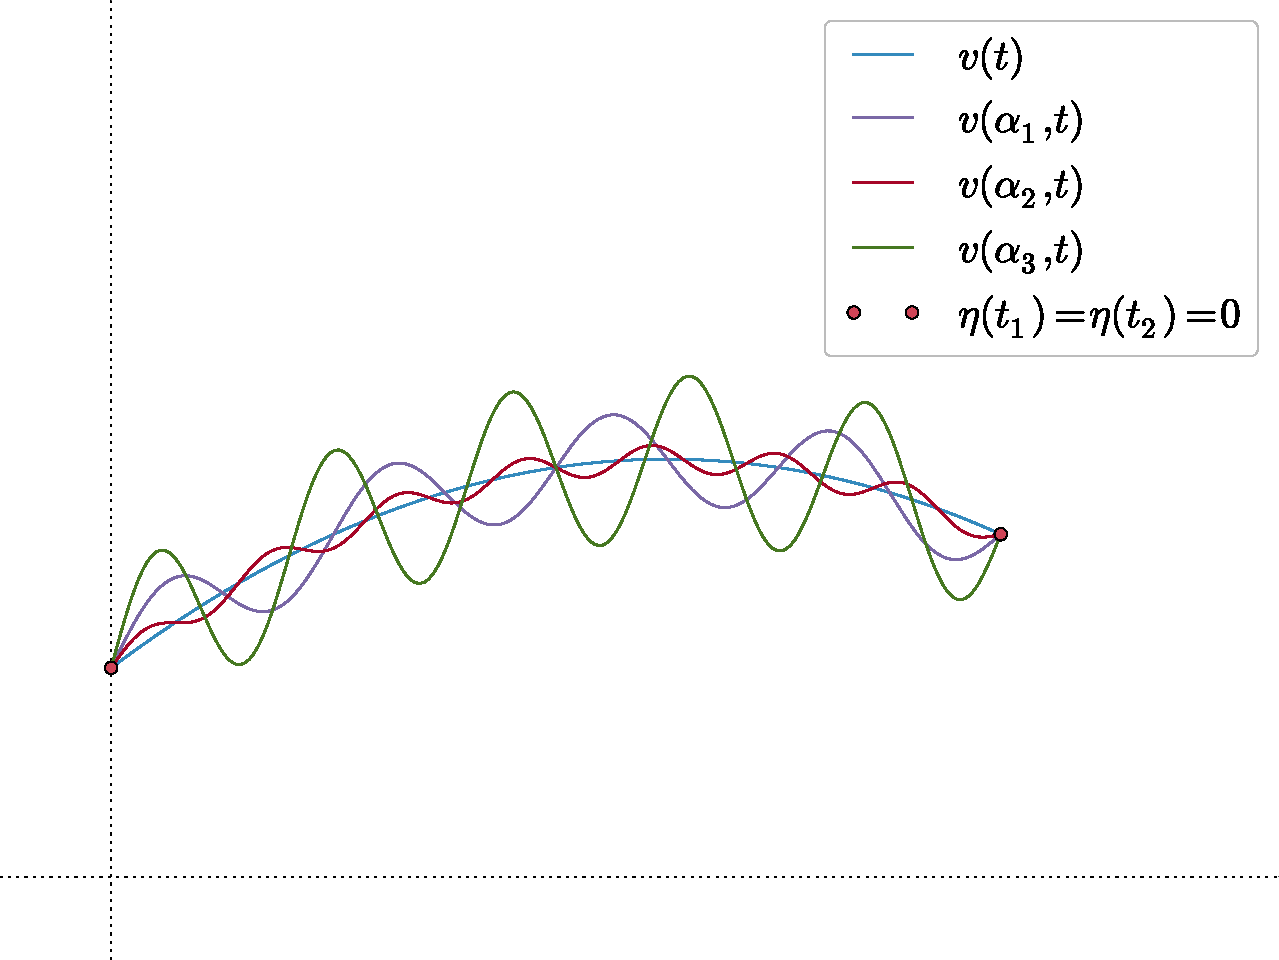
\includegraphics[width=0.7\textwidth]{./imagenes/trayectorias.pdf}
        \caption{\label{fig:trayectorias}Trayectorias $v(\alpha, t)$ solución para $J(v(t), v'(t))$.}
    \end{figure}

    es decir $\eta(t_1) = \eta(t_2) = 0$, pero además $\eta(t) \in e^1$.\footnote{Si $f \in e^1$, $f$ es una función diferenciable al menos una vez.}

    Con esta parametrización en $\alpha$:

    \begin{equation*}
        v(t) \to v(\alpha, t) = v(0, t) + \alpha \eta(t)
    \end{equation*}

    tenemos que la ecuación~\ref{eq:opfun1} nos queda:

    \begin{equation*}
        J(\alpha) = \int_{t_1}^{t_2} f_1(v(\alpha, t), v'(\alpha, t), t) dt
    \end{equation*}

    donde tenemos que $\alpha = 0$ implica que $J$ es un extremo y $\alpha \ne 0$ implica que $J$ no es un extremo.

    Debido a esto, podemos concluir que $J$ tambien esta parametrizada de esta manera:

    \begin{equation*}
        J \to J(\alpha)
    \end{equation*}

    La condición necesaria para que $J$ tenga un valor estacionario (extremo), es que $J$ sea independiente de $\alpha$ en primer orden (que este relacionado linealmente), a lo largo de la trayectoria que otorga el extremo ($\alpha = 0$), es decir:

    \begin{equation}
        \left. \frac{\partial J}{\partial \alpha} \right|_{\alpha=0} = 0 \quad \forall \eta \in e^1
    \end{equation}

    \begin{nota}
        Observe que solo es una condición necesaria, es decir:

        \begin{equation*}
            J \text{ es extremo } \implies \left. \frac{\partial J}{\partial \alpha} \right|_{\alpha=0} = 0
        \end{equation*}
    \end{nota}

    \newpage
    \section{Ecuación de Euler}

    La condición necesaria es:

    \begin{equation*}
        \left. \frac{\partial J}{\partial \alpha} \right|_{\alpha=0} = 0
    \end{equation*}

    entonces hay que seguir los siguientes pasos:

    \begin{enumerate}
        \item Calcular $\frac{\partial J}{\partial \alpha}$.
        \item Hacer $\alpha = 0$.
    \end{enumerate}

    Empecemos calculando la derivada parcial de $J$:

    \begin{multline*}
        \frac{\partial J}{\partial \alpha} = \frac{\partial}{\partial \alpha} \int_{t_1}^{t_2} f_1(v(\alpha, t), v'(\alpha, t), t)dt = \\
        \int_{t_1}^{t_2}\left( \frac{\partial f_1(\dots)}{\partial v(\alpha, t)} \frac{\partial v(\alpha, t)}{d \alpha} + \frac{\partial f_1(\dots)}{\partial v'(\alpha, t)} \frac{\partial v'(\alpha, t)}{d \alpha} \right) dt
    \end{multline*}

    en este punto aparecen términos reducibles:

    \begin{equation*}
        \frac{\partial v(\alpha, t)}{\partial \alpha} = \frac{\partial v(t)}{\partial \alpha} + \frac{\partial \left(\alpha \eta(t) \right)}{\partial \alpha} = \eta(t)
    \end{equation*}

    \begin{equation*}
        \frac{d v'(\alpha, t)}{d\alpha} = \frac{\partial}{\partial \alpha} \left( \frac{d v(\alpha, t)}{dt} \right) = \frac{\partial}{\partial \alpha} \left( v'(t) + \alpha \frac{d \eta(t)}{dt} \right) = \frac{d \eta(t)}{dt}
    \end{equation*}

    lo que nos deja:

    \begin{equation*}
        \frac{\partial J}{\partial \alpha} = \int_{t_1}^{t_2}\left( \frac{\partial f_1(\dots)}{\partial v(\alpha, t)} \eta(t) + \frac{\partial f_1(\dots)}{\partial v'(\alpha, t)} \frac{d \eta(t)}{dt} \right) dt
    \end{equation*}

    la segunda parte de esta integral es integrable por partes, si hacemos $u = \frac{\partial f_1(\dots)}{\partial v'(\alpha, t)}$, $dv = \frac{d\eta(t)}{dt}dt$, $du = \frac{d}{dt}\left( \frac{\partial f_1(\dots)}{dv'(\alpha, t)} \right)$ y $v = \eta(t)$:

    \begin{equation*}\frac{\partial J}{\partial \alpha} = \int_{t_1}^{t_2}\left( \frac{\partial f_1(\dots)}{\partial v(\alpha, t)} \eta(t) - \frac{d}{dt} \left( \frac{\partial f_1(\dots)}{\partial v'(\alpha, t)} \right) \eta(t) \right) dt + \left. \frac{\partial f_1(\dots)}{\partial v'(\alpha, t)} \eta(t) \right|_{t_1}^{t_2}
    \end{equation*}

    pero recordemos que $\eta(t_1) = \eta(t_2) = 0$, por lo que el ultimo termino se elimina y nos queda:

    \begin{multline} \label{eq:opfun2}
        \frac{\partial J}{\partial \alpha} = \int_{t_1}^{t_2}\left( \frac{\partial f_1(\dots)}{\partial v(\alpha, t)} \eta(t) - \frac{d}{dt} \left( \frac{\partial f_1(\dots)}{\partial v'(\alpha, t)} \right) \eta(t) \right) dt = \\
        \int_{t_1}^{t_2}\left( \frac{\partial f_1(v(\alpha, t), v'(\alpha, t), t)}{\partial v(\alpha, t)} - \frac{d}{dt} \left( \frac{\partial f_1(v(\alpha, t), v'(\alpha, t), t)}{\partial v'(\alpha, t)} \right) \right) \eta(t) dt
    \end{multline}

    Si ahora, en la ecuación~\ref{eq:opfun2} sustituimos $\alpha = 0$, obtendremos:

    \begin{equation*}
        \left. \frac{\partial J}{\partial \alpha} \right|_{\alpha=0} = \int_{t_1}^{t_2}\left( \frac{\partial f_1(v(t), v'(t), t)}{\partial v(t)} - \frac{d}{dt} \left( \frac{\partial f_1(v(t), v'(t), t)}{\partial v'(t)} \right) \right) \eta(t) dt
    \end{equation*}

    Por lo que la condición necesaria es:

    \begin{equation*}
        \int_{t_1}^{t_2}\left( \frac{\partial f_1(v(t), v'(t), t)}{\partial v(t)} - \frac{d}{dt} \left( \frac{\partial f_1(v(t), v'(t), t)}{\partial v'(t)} \right) \right) \eta(t) dt = 0 \quad \forall \eta(t) \in e^1
    \end{equation*}

    lo cual implica que:

    \begin{equation}
        \frac{\partial f_1(v(t), v'(t), t)}{\partial v(t)} - \frac{d}{dt} \left( \frac{\partial f_1(v(t), v'(t), t)}{\partial v'(t)} \right)  = 0
    \end{equation}

    esta es la que conocemos como ecuación de Euler.

    \newpage
    \section{Multiplicadores de Lagrange}

    Deseamos resolver el siguiente problema:

    Minimizar la función
    $f(v):\mathbbm{R}^n \to \mathbbm{R}$
    sujeta a la restricción $\mathscr{G}(v) = 0$
    , donde $\mathscr{G}(v)=\begin{pmatrix}\mathscr{G}_1(v) & \mathscr{G}_2(v) & \dots & \mathscr{G}_m(v) \end{pmatrix} \in \mathbbm{R}^m$
     y $\mathscr{G}_i(v): \mathbbm{R}^n \to \mathbbm{R}$
     con $i \in \left\{ 1, 2, \dots, m \right\}$.

    Para resolver este problema haremos uso de los multiplicadores de Lagrange, los cuales estan basados en el concepto de la derivada direccional\footnote{Esta derivada es formalmente conocida como la derivada de Fréchet, la cual se relaciona linealmente con la diferencial de Fréchet.}

        \subsection{Derivada direccional y vector gradiente}

        \begin{definicion}
            La derivada direccional de $f_1$ en $v_0 \in \mathbbm{R}^n$ en la dirección del vector unitario $\eta \in \mathbbm{R}^n$ es:

            \begin{equation}
                D_{\eta} f_1(v_0) = \lim_{\alpha \to 0}^{n}  \frac{f_1(v_0 + \alpha) - f_1(v_0)}{\alpha}
            \end{equation}

            donde $\alpha$ es un escalar, es decir, $\alpha \in \mathbbm{R}$, en el caso de que este limite exista.

            \missingfigure{Superficie con vector posición evaluado y vector dirección de la derivada unitario.}

            \missingfigure{Curva cortada por una recta por la que pasa un vector restando los dos puntos evaluados de la curva.}

            Esta derivada nos da la razon de cambio de $f_1$ en el punto $v_0$ y en la dirección $\eta$, siempre y cuando $\alpha \to 0$.
        \end{definicion}

        \begin{teorema}
            Si $f_1$ es una función diferenciable de $v \in \mathbbm{R}^n$, entonces $f_1$ tiene una derivada direccional en la dirección de cualquier vector unitario $\eta \in \mathbbm{R}^n$ y por lo tanto:

            \begin{equation}
                D_{\eta} f_1(v) = \sum_{i=1}^n \frac{\partial f_1(v_i)}{dv_i} \eta_i
            \end{equation}

            donde $v = \begin{pmatrix} v_1 \\ v_2 \\ \vdots \\ v_n \end{pmatrix} \in \mathbbm{R}^n$, $\eta = \begin{pmatrix} \eta_1 \\ \eta_2 \\ \vdots \\ \eta_n \end{pmatrix} \in \mathbbm{R}^n$ con $|| \eta || = 1$.
        \end{teorema}

        \begin{definicion}
            Dada una base ortonormal de $\mathbbm{R}^n$, $\left\{ e_1, e_2, \dots, e_n \right\}$, entonces el gradiente de $t_1$ es la función vectorial, $\nabla f_1$, definida por:

            \begin{equation} \label{eq:opfun3}
                \nabla_v f_1(v) = \sum_{i=1}^n \frac{\partial f_1}{\partial v_i} e_i
            \end{equation}

            donde $v_i = \sum_{i=1}^n v_i e_i$.
        \end{definicion}

        Con esta notación gradiente, la ecuación~\ref{eq:opfun3} de la derivada direccional se escribe:

        \begin{equation}
            D_{\eta} f_1(v) = \left( \nabla f_1(v), \eta \right)
        \end{equation}

        donde $\left( R, S \right): \mathbbm{R}^n \times \mathbbm{R}^n \to \mathbbm{R}$ es el producto punto, es decir, la proyección escalar del vector $R$ sobre la dirección del vector $S$.

        \begin{teorema}
            Suponga que $f_1: \mathbbm{R}^n \to \mathbbm{R}$ es una funcional diferenciable. El máximo valor de la derivada $D_{\eta}f(v)$ es $||D_{\eta}f(v)||$ y se obtiene cuando la dirección de $\eta$ coincide con el vector gradiente $\nabla_v f_1(v)$.
        \end{teorema}

        Sea la superficie, $\mathscr{S}$, definida por la funcional $\mathscr{G}:\mathbbm{R}^n \to \mathbbm{R}$ de la siguiente manera:

        \begin{equation}
            \mathscr{S} = \left\{ v \in \mathbbm{R}^n \mid \mathscr{G}(v) = k \right\}
        \end{equation}

        Sea $\mathscr{C}$ una curva contenida en $\mathscr{S}$ y que pase por el punto $v_0 \in \mathbbm{R}$, la cual está definida por la función vectorial $R: \mathbbm{R} \to \mathbbm{R}^n$, esto es:

        \begin{equation}
            \mathscr{C} = \left\{ v \in \mathbbm{R}^n, t \in \mathbbm{R} \mid v = R(t)\right\}
        \end{equation}

        Sea $t_0 \in \mathbbm{R}$ tal que $R(t_0) = v_0$.

        Como $\mathscr{C} \subset \mathscr{S}$, entonces cualquier punto, $v \in \mathscr{C}$, satisface:

        \begin{equation*}
            \mathscr{G}(v) = k
        \end{equation*}

        lo cual implica (asumiendo que $v$ es una función diferenciable y que tambien $\mathscr{G}$ lo es):

        \begin{equation*}
            \sum_{i=1}^n \frac{\partial \mathscr{G}}{\partial v_i} \frac{d v_i}{dt} = 0
        \end{equation*}

        es decir:

        \begin{equation*}
            \left( \nabla_i \mathscr{G}, R'(t) \right) = 0
        \end{equation*}

        donde $R'(t) = \frac{dR(t)}{dt} = \begin{pmatrix} \frac{d v_1(t)}{dt} \\ \frac{d v_2(t)}{dt} \\ \vdots \\ \frac{d v_n(t)}{dt} \end{pmatrix} \in \mathbbm{R}^n$.

        En particular, cuando $t = t_0$, se tiene:

        \begin{equation*}
            R(t_0) = v_0
        \end{equation*}

        \begin{equation*}
            \left( \nabla_v \mathscr{G}(v_0), \frac{dR(t_0)}{dt} \right) = 0
        \end{equation*}

        Esta ecuación indica que el vector gradiente en $v_0$, $\nabla_v \mathscr{G}(v_0)$,  es perpendicular al vector tangente $\frac{dR(t_0)}{dt}$ a cualquier $\mathscr{C} \subset \mathscr{S}$ que pase por $v_0$.

        \missingfigure{Superficie con vector tangente.}

        \missingfigure{Plano tangente a superficie de nivel y vector normal al plano.}

        Si $\nabla_v \mathscr{G}(v_0) \ne 0$, entonces se define el plano tangente a la superficie de nivel $\mathscr{S}$, en el punto $\mathscr{G}(v_0)$ y tiene un vector normal $\nabla_v \mathscr{G}(v_0)$, esto es, el plano tangente $\tau$ que esta definido por:

        \begin{equation}
            \tau = \left\{ v \in \mathbbm{R}^n \mid \left( \nabla_v \mathscr{G}(v_0), v - v_0 \right) = 0 \right\}
        \end{equation}

        \newpage
        \section{Multiplicadores de Lagrange}

        Procederemos ahora a resolver el problema original. Suponga que la funcional $f_1$ tiene un extremo en el punto $v_0$ en la superficie:

        \begin{equation}
            \mathscr{S}_m \left\{ v \in \mathbbm{R}^n, i \in \left\{ 1, 2, \dots, m \right\} \mid \mathscr{G}(v) = 0 \right\}
        \end{equation}

        donde $\mathscr{G}(v) = \begin{pmatrix} \mathscr{G}_1(v) \\ \mathscr{G}_2(v) \\ \vdots \\ \mathscr{G}_m(v) \end{pmatrix} \in \mathbbm{R}^m$
            y $\mathscr{G}_i(v):\mathbbm{R}^n \to \mathbbm{R}$
            con $i \in \left\{ 1,2,\dots,m \right\}$.

        Sea una curva:

        \begin{equation}
            \mathscr{C} = \left\{ v\in \mathbbm{R}^n t \in \mathbbm{R} \mid v = R(t) \right\} \subset \mathscr{S}_m
        \end{equation}

        tal que $v_0 \in \mathscr{C}$.

        Sea $t_0 \in \mathbbm{R}$ el paramtero correspondiente a $v_0$, es decir $v_0 = R(t_0)$.

        La funcional compuesta:

        \begin{equation}
            \mathscr{H} = f_1(R(t))
        \end{equation}

        representa a los valores de $f$  que también está en $\mathscr{C}$.

        Como $f_1$ tiene un extremo en $v_0$, entonces $\mathscr{H}$ tiene un extremo en $t_0$, por lo que:

        \begin{equation}
            \left. \frac{d \mathscr{H}(t)}{dt} \right|_{t=t_0} = 0
        \end{equation}

        Pero si $f$ es diferenciable, se deduce por la regla de la cadena:

        \begin{equation}
            0 = \left. \frac{d}{dt} \mathscr{H} \right|_{t=t_0} = \left. \sum_{i=1}^n \frac{\partial f_1}{\partial v_i} \frac{v_i(t)}{dt} \right|_{t=t_0, v=v_0} = \left( \nabla_v f_1(v_0), \frac{d}{dt} R(t_0) \right)
        \end{equation}

        esto nos indica que el vector gradiente $\nabla_v f_1(v_0)$, es ortogonal al vector tangente, $\frac{d R(t_0)}{dt}$, para cada una de estas curvas.

        Pero sabemos que los vectores gradientes de las coordenadas, $\left( \mathscr{G}_i, \mathscr{G}_i(v_0) \right)$, son tambien ortogonales a $\frac{d R(t_0)}{dt}$, por lo que los vectores gradiente $\nabla_v f_1(v_0)$ y $\nabla_v \mathscr{G}_i(v_0)$ con $i \in \left\{ 1, 2, \dots, m \right\}$ necesariamente son paralelos.

        Entonces, si $\nabla_v \mathscr{G}_i(v_0)$ con $i \in \left\{ 1, 2, \dots, m \right\}$, existen $\lambda_1, \lambda_2, \dots, \lambda_m$, tales que:

        \begin{equation}
            \nabla_v f_1(v_0) = \sum_{i=1}^m \lambda_i \nabla_v \mathscr{G}_i(v_0)
        \end{equation}

        y al vector $\lambda = \begin{pmatrix} \lambda_1 \\ \lambda_2 \\ \vdots \\ \lambda_m \end{pmatrix} \in \mathbbm{R}^m$ se le conoce como multiplicadores de Lagrange.

        Entonces para resolver el problema original se procede como sigue:

        \begin{enumerate}
            \item Se construye la siguiente funcional aumentada:

            \begin{equation}\label{eq:opfun3}
                f_a(v, \lambda) = f_1(v) - \left( \lambda, \mathscr{G}(v) \right)
            \end{equation}

            \item Se encuentran los puntos estacionarios de la ecuación~\ref{eq:opfun3}:

            \begin{eqnarray}\label{eq:opfun4}
                \nabla_v f_a(v, \lambda) & = & 0 \nonumber \\
                \nabla_\lambda f_a(v, \lambda) & = & 0
            \end{eqnarray}
        \end{enumerate}

        El par $(v_0, \lambda_0)$ que satisface la ecuación~\ref{eq:opfun4} es la solución del problema original.

        Observe que con este método, se esta transformando un problema de optimización con restricciones, en uno sin restricciones.


    \clearpage
    \chapter{Introducción al control óptimo}

    Sea el sistema descrito por la representación de estado:

    \begin{equation} \label{eq:conop1}
        \frac{dx}{dt} = A x + b u
    \end{equation}

    donde $A \in \mathbbm{R}^{n \times n}$, $b \in \mathbbm{R}^{n \times n}$, con condiciones iniciales $x(0) = x_0 \in \mathbbm{R}^n$; se desea minimizar el indice de desempeño:

    \begin{equation} \label{eq:conop2}
        J(x, u) = \frac{1}{2} \int_0^{\infty} \left( x^T Q x + \rho u^2 \right) dt
    \end{equation}

    donde $\rho > 0$ y $Q = Q^T \ge 0$, a lo largo de las trayectorias solución de la ecuación~\ref{eq:conop1}. Es decir se desea minimizar la ecuación~\ref{eq:conop2} con las restricciones de la ecuación~\ref{eq:conop1}.

    Este problema de minimización con restricciones se va a resolver usando los multiplicadores de Lagrange.

    El indice de desempeño aumentado es:

    \begin{equation*}
        Ja(x, u, \lambda) = \int_0^{\infty} \left( \frac{1}{2}  \left( x^T Q x + \rho u^2 \right) + \lambda^T \left( Ax + bu - \frac{dx}{dt} \right) \right)
    \end{equation*}

    Definiendo los siguientes funcionales:

    \begin{description}
        \item [Lagrangiano]
        \begin{equation}
            \mathscr{L}(x, u, \lambda, t) = \frac{1}{2} \left( x^T Q x + \rho u^2 \right)
        \end{equation}
        \item [Hamiltoniano]
        \begin{equation}
            \mathscr{H}(x, u, \lambda, t) = \mathscr{L}(x, u, \lambda, t) + \lambda^T (A x + b u)
        \end{equation}
    \end{description}

    se obtiene:

    \begin{equation}
        Ja(x, u, \lambda) = \int_0^{\infty} \left( \mathscr{H}(x, u, \lambda, t) - \lambda^T \dot{x} \right) dt
    \end{equation}

    si tenemos que $v =\begin{pmatrix} x \\ u \\ \lambda \end{pmatrix}$, podemos ver al indice de desempeño aumentado como una función:

    \begin{equation*}
        Ja(x, u, \lambda) = \int_0^{\infty} f(v, \dot{v}, t) dt
    \end{equation*}

    Sabemos que la ecuación de Euler es:

    \begin{equation}
        \frac{\partial f(v, \dot{v}, t)}{\partial v} - \frac{d}{dt} \left( \frac{\partial f(v, \dot{v}, t)}{\partial \dot{v}} \right) = 0
    \end{equation}

    pero sabemos que $v$ es un vector con 3 funciones, por lo que al derivar con respecto a cada una tendremos:

    \begin{enumerate}
        \item Con respecto a $x$:

        \begin{eqnarray*}
            \frac{\partial f}{\partial x} - \frac{d}{dt} \left( \frac{\partial f}{\partial \dot{x}} \right) & = & 0 \\
            \frac{\partial \mathscr{H}}{\partial x} - \frac{d}{dt} \left( -\lambda \right) & = & 0 \\
            Q x + A^T \lambda + \frac{d \lambda}{dt} & = & 0
        \end{eqnarray*}

        lo cual implica:

        \begin{equation} \label{eq:conop3}
            - \frac{d \lambda}{dt} = Q x + A^T \lambda
        \end{equation}

        \item Con respecto a $u$:

        \begin{eqnarray*}
            \frac{\partial f}{\partial u} - \frac{d}{dt} \left( \frac{\partial f}{\partial \dot{u}} \right)  & = & 0 \\
            \frac{\partial \mathscr{H}}{\partial u} - \frac{d}{dt} \left( 0 \right) & = & 0 \\
            \rho u + \lambda^T b & = & 0
        \end{eqnarray*}

        lo cual implica:

        \begin{equation} \label{eq:conop4}
            u = - \rho^{-1} b^T \lambda
        \end{equation}

        \item Con respecto a $\lambda$:

        \begin{eqnarray*}
            \frac{\partial f}{\partial \lambda} - \frac{d}{dt} \left( \frac{\partial f}{\partial \dot{\lambda}} \right) & = & 0 \\
            \frac{\partial \mathscr{H}}{\partial \lambda} - \frac{dx}{dt} - \frac{d}{dt} \left( 0 \right) & = & 0 \\
            A x + b u -\frac{dx}{dt} = 0
        \end{eqnarray*}

        lo cual implica:

        \begin{equation} \label{eq:conop5}
            \frac{dx}{dt} = A x + b u
        \end{equation}
    \end{enumerate}

    De las ecuaciones~\ref{eq:conop3},~\ref{eq:conop4} y~\ref{eq:conop5} podemos obtener el siguiente resultado:

    \begin{equation} \label{eq:conop6}
        \begin{pmatrix}
            \dot{x} \\
            \dot{\lambda}
        \end{pmatrix} =
        \begin{pmatrix}
            A & -b \rho^{-1} b^T \\
            - Q & - A^T
        \end{pmatrix}
        \begin{pmatrix}
            x \\
            \lambda
        \end{pmatrix}
    \end{equation}

    de donde $M = \begin{pmatrix} A & -b \rho^{-1} b^T \\ - Q & - A^T \end{pmatrix}$ es la matriz de Hamilton, y las condiciones de frontera del sistema son $x(0) = x_0$ y $\lim_{t \to \infty} \lambda(t) = 0$.

    Si bien hemos usado a $\lambda$, aun no hemos mencionado que esta variable representa el coestado del sistema y si bien las condiciones de frontera del sistema son correctas, cabe mencionar que lo que realmente queremos es que $x(0) = x_0$ y $\lim_{t \to \infty} x(t) = 0$, por lo que hace falta relacionar al estado del sistema, $x(t)$, con el coestado, $\lambda(t)$.

    En base a la ecuación~\ref{eq:conop4} se propone que la solución sea una realimentación de estado, para esto se propone que el estado $x$ y el coestado $\lambda$ esten relacionados por una matriz $P$, esto es:

    \begin{equation} \label{eq:conop7}
        \lambda = P x
    \end{equation}

    Por lo que de las ecuaciones~\ref{eq:conop6} y~\ref{eq:conop7}, podemos obtener que:

    \begin{equation*}
        \begin{pmatrix}
            I \\
            P
        \end{pmatrix} \dot{x}=
        \begin{pmatrix}
            A & -b \rho^{-1} b^T \\
            - Q & - A^T
        \end{pmatrix}
        \begin{pmatrix}
            I \\
            P
        \end{pmatrix} x
    \end{equation*}

    si premultiplicamos esta expresión con $\begin{pmatrix} P & -I \end{pmatrix}$, obtendremos:

    \begin{equation*}
        0 =
        \begin{pmatrix}
            P A + Q & -P b \rho^{-1} b^T + A^T
        \end{pmatrix}
        \begin{pmatrix}
            I \\
            P
        \end{pmatrix} x
    \end{equation*}

    \begin{equation*}
        0 = \left( A^T P + P A - P b \rho^{-1} b^T P + Q \right) x \quad \forall x \text{ solución del sistema~\ref{eq:conop1}}
    \end{equation*}

    Por lo que hemos llegado a la ecuación algebraica de Riccati:

    \begin{equation} \label{eq:conop8}
        A^T P + P A - P b \rho^{-1} b^T P + Q = 0
    \end{equation}

    siendo la ley de control óptimo (de las ecuaciones~\ref{eq:conop4} y~\ref{eq:conop7}):

    \begin{equation} \label{eq:conop9}
        u = -f_*^T
    \end{equation}

    donde $f_*^T = \rho^{-1} b^T P$.

    Note que de las ecuaciones~\ref{eq:conop8} y~\ref{eq:conop9}, se obtiene la ecuación de Lyapunov del sistema en lazo cerrado:

    \begin{eqnarray}
        A^T P + P A - P b f_*^T & = & -Q \nonumber \\
        A^T P + P \left( A - b f_*^T \right) & = & - Q \nonumber \\
        \left( A - b f_*^T \right)^T P + P \left( A - b f_*^T \right) & = & - \left( Q + f_* b^T P \right) \nonumber \\
        \left( A - b f_*^T \right)^T P + P \left( A - b f_*^T \right) & = & - \left( Q + f_* \rho f_*^T \right)
    \end{eqnarray}

    En donde la expresión del lado derecho debe ser $\left( Q + f_* b^T P \right) = \left( Q + f_* b^T P \right)^T \ge 0$, por lo que tambien pediremos que $P$ sea simétrica y semidefinida positiva ($P = P^T \ge 0$).

    Como nota final, tan solo hacemos notar que el sistema realimentado queda:

    \begin{equation}
        \frac{dx}{dt} = (A - b f_*^T) x
    \end{equation}

    Y que una manera gráfica de interpretar la minimización del indice de desempeño es de manera grafica.

    \missingfigure{Trayectoria del comportamiento del sistema a traves del tiempo.}


\end{document}
